% !TeX root = dissertation.tex
\chapter{Recommending Privacy Settings for Fitness IoT}\label{chapter:fitnessIoT}

\section{Introduction}\label{fitnessIntro}
In Chapter~\ref{chapter:generalIoT} and~\ref{chapter:householdIoT}, we have discussed how we apply the data-driven approach to the general/public IoT and household IoT contexts, respectively. We developed corresponding IoT privacy-setting interface prototypes that integrated with smart defaults/profiles by predicting users' privacy decisions. In this chapter, we present the work we did in the domain of fitness IoT. We further test the previously-developed data-driven approach to design privacy-setting interfaces for users of fitness IoT devices. Note that moving the context from general/public IoT to household IoT, now to fitness IoT, the context that we are focusing is becoming more narrow. The change of environment brought more challenge. For example, now for fitness IoT, there is no contextual scenario existing, which we focused on in Chapter~\ref{chapter:generalIoT} and~\ref{chapter:householdIoT}. Considering almost all the current fitness IoT devices require corresponding mobile Apps to be used together and the mobile Apps are usually the ones who are take charge of users' privacy information, we focus on the privacy permissions asked by the mobile Apps. In this Chapter, we first collect users permission decisions to the fitness IoT permissions. Then we apply our data-driven approach to classify users into groups based on their permission decisions, and create permission profiles for each groups. This allows new users to answer very few questions before getting a recommendation of a set of permission profile, which simplifies users' task of setting every permission for fitness IoT devices.

%As fitness-related data are persistently captured, stored, processed and shared by these devices and related services, the issue of privacy management is becoming increasingly urgent both for the user and the service, which has to respect privacy law, including the new European Union's General Data Protection Regulation (GDPR). This concerns all third parties that manage user data and has of course a major impact on personalization services.

%As of May 25, 2018, the European Union (EU) enforce the General Data Protection Regulation (GDPR)~\cite{ref:GDPR} which applies to the storage, processing and use of the subject's personal data from the third parties which may or may not have been established in the EU as long as they operate in an EU market or acess data of EU residents. It requires users to provide explicit consent to privacy options expressed by third parties. This results in a complex task for the users given the number of devices and applications which have to be read and processed specifically.

\section{Data Model}
As discussed in Section~\ref{fitnessIntro}, the mechanism that most modern fitness trackers use to guide their user to manage privacy settings is by asking users various permission questions. We first investigate the questions asked by mainstream fitness trackers, and then adapt those questions for the use of our data model in this study.

As shown in Figure~\ref{tab:trackerspermission}, we examined the permission questions asked by the mainstream fitness trackers (Fitbit, Garmin, Jawbone, and Misfit) and categorized these questions into 3 groups -- \textit{Smartphone Persmission}, \textit{In-app Requests}, and \textit{Fitness Data},.
 
\begin{figure*}
	\centering
	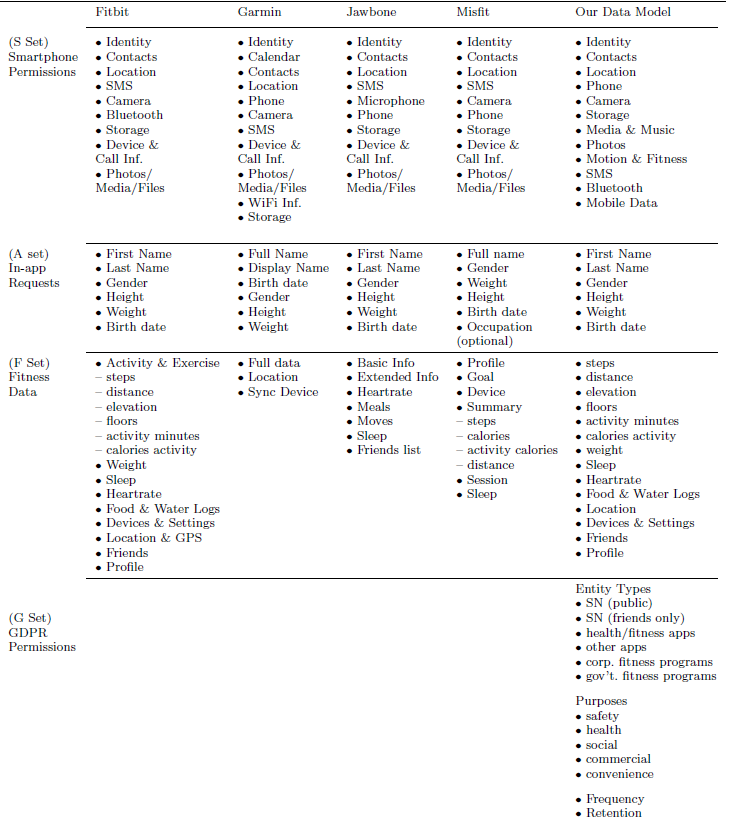
\includegraphics[width=\textwidth]{figures/fitnessCompare.png}
	\caption{Comparison of permissions asked by Fitness Trackers and the fitness IoT Data Model used for this study.}
	\label{tab:trackerspermission}
\end{figure*}

\subsection{Smartphone Permissions (S set)}
The first group of permissions are the smartphones permissions, which are requested during the installing or the first use of the mobile application. The requested smartphone permissions differs by the brands of the fitness trackers as well as the mobile Operation System of the smartphones. As shown in Figures~\ref{fig:iosS} and~\ref{fig:androidS}, even for the mobile application from the same manufacturer (Fitbit), the requested smartphone permissions are different between the iOS version and the Android version. We summarize all the requested smartphone permissions by popular brands of fitness trackers' mobile application across different mobile Operating Systems (i.e. iOS, Android, and Windows Mobile).

\begin{figure}
	\centering
	\begin{subfigure}[b]{0.48\linewidth}
		\centering
		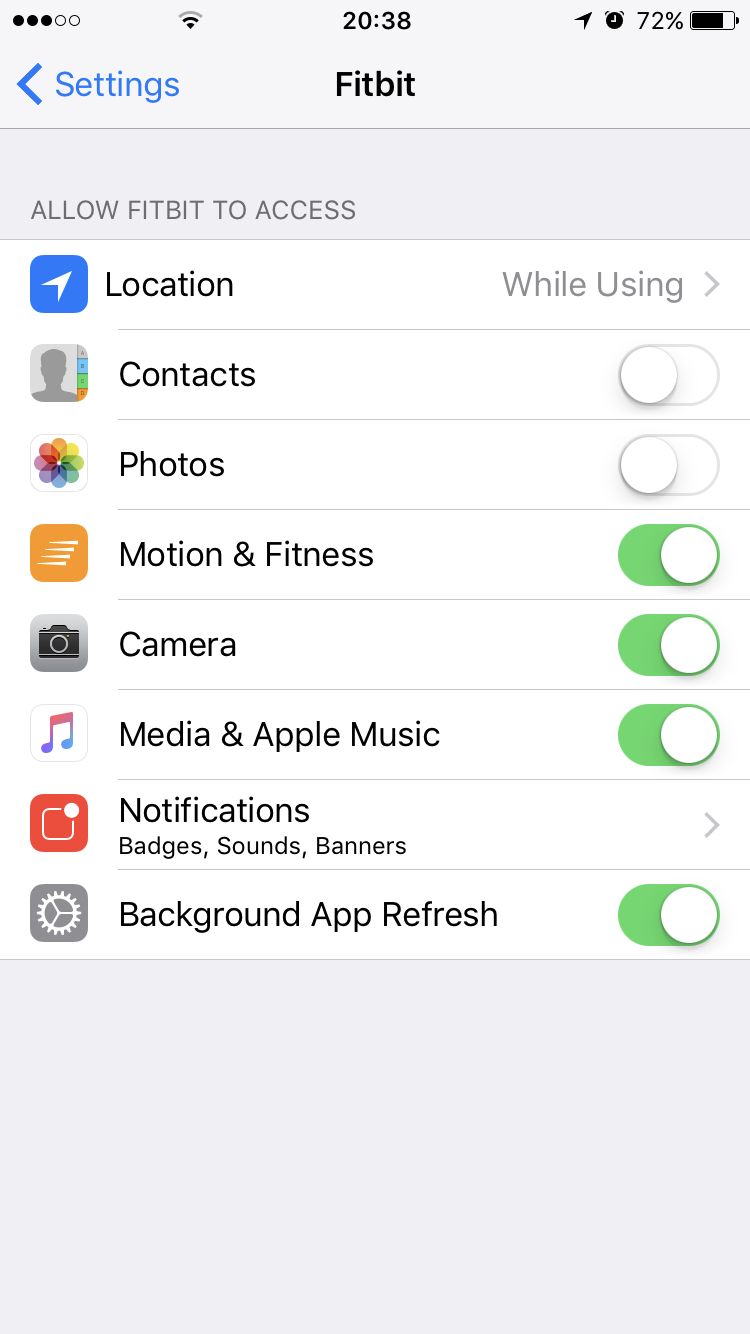
\includegraphics[width=120pt]{figures/ios.png}
		\caption{The interface of smartphone permissions of Fitbit iOS App}
		\label{fig:iosS}
	\end{subfigure}%
	\begin{subfigure}[b]{0.48\linewidth}
		\centering
		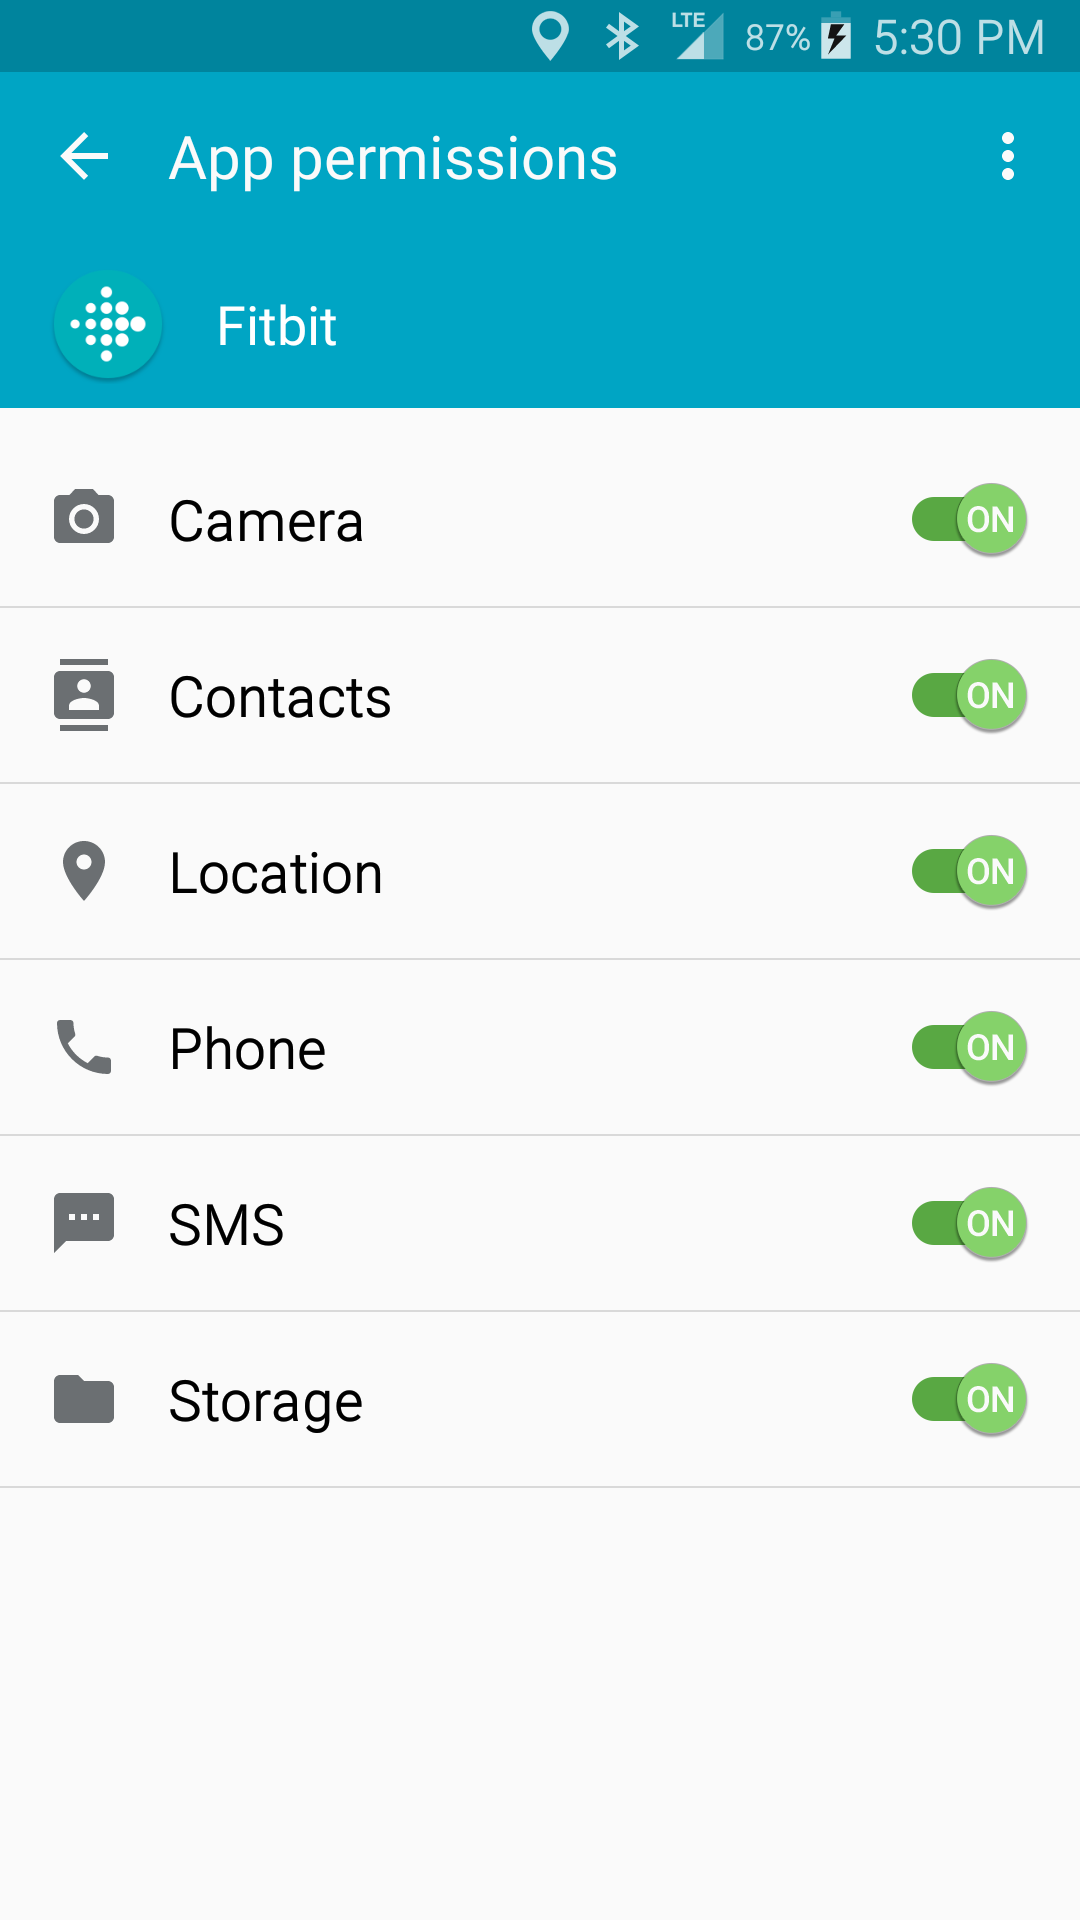
\includegraphics[width=120pt]{figures/android6.png}
		\caption{The interface of smartphone permissions of Fitbit Android App}
		\label{fig:androidS}
	\end{subfigure}
	\caption{Interface examples of Smartphone Permissions requests for Fitbit trackers (S set)}
	%\caption{\subref{fig:iosS} shows Figure~1 and~\subref{fig:androidS} shows Figure~2.}
\end{figure}

\subsection{In-App Requests (A set)}
Fitness tracks also intend to collect user's data in their mobile applications. For example, Fitbit asks users to provide their \textit{First Name}, \textit{Last Name}, \textit{Gender}, \textit{Height}, \textit{Weight}, \textit{Birth Date}, as shown in Figure~\ref{fig:fitbitA} when signing up an account during the first-time using the mobile App. Note that these data are mandatory for all fitness trackers in Figure~\ref{tab:trackerspermission}; the only optional piece of information is Misfit's request on users' occupation. Figure~\ref{fig:fitbitA} shows the \emph{A set} for the Fitbit app (other apps are similar).
\begin{figure}
	\centering
	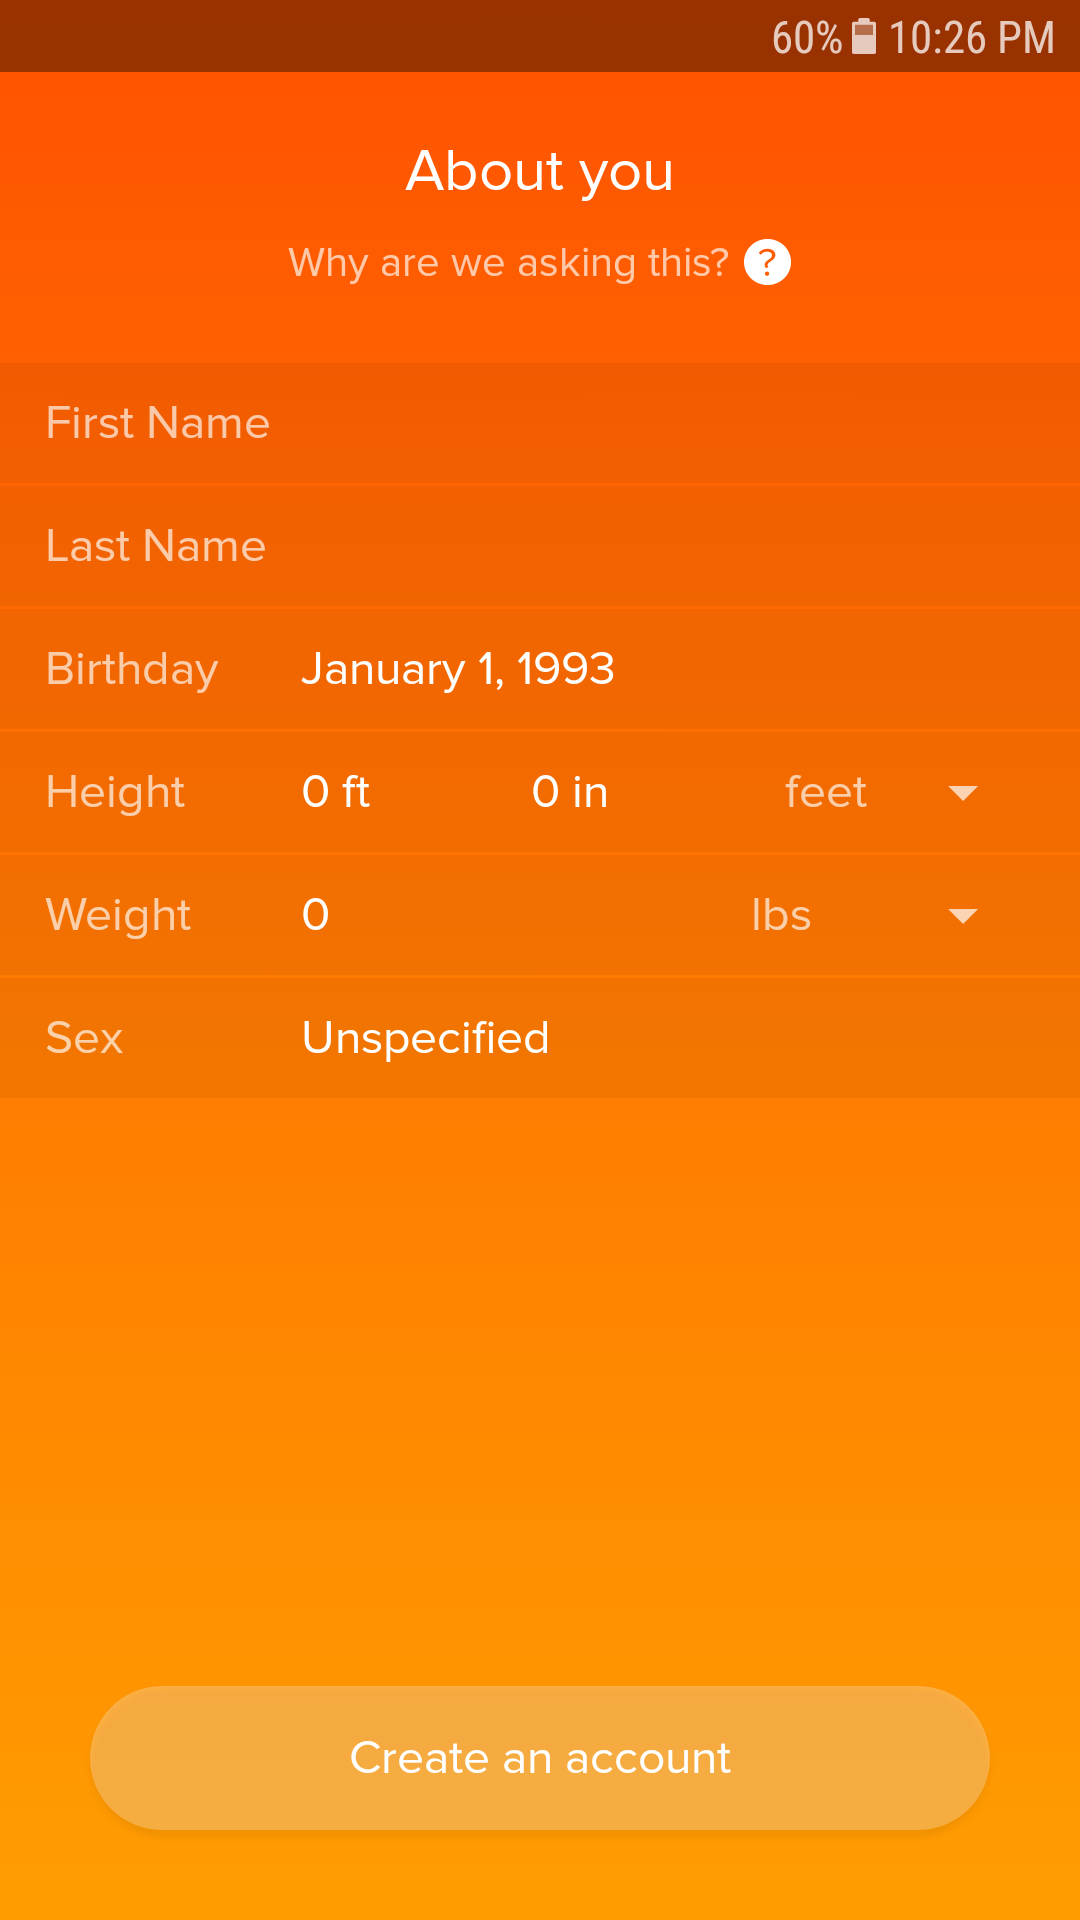
\includegraphics[width=0.2\textheight]{figures/Aset.png}
	\caption{Interface example of In-App Permissions requests in Fitbit Android App (A set)}
	\label{fig:fitbitA}
\end{figure}

\subsection{Fitness Data Permissions (F set)}
\label{sec:fset}
F set contains fitness-related data that is either automatically collected by the fitness tracker or manually input by the users, such as food and water logs, friend list. As shown in Figure~\ref{tab:trackerspermission}, we follow Fitbit's permission model for F set but give users more fine-grained control over \textit{Activity and Exercise} data by breaking these permissions down into steps, distance, elevation, floors, activity minutes, and calories activity. A total of 14 permissions are included in the F set for our study. 

%NEW
%new: according to Prof. Bart, explain the F-G connection
%Note that the F set permissions are repeated for \emph{each additional TP} that requests access to this data. As such, these permissions are not for the native app of the fitness tracker, but for other TP apps that the user desires to use and allow access to her/his fitness tracking data. In this study, instead of taking into account individual third parties, we use the PPIoT \textit{EntityType}, discussed in Section \ref{sec:ppiot}, to investigate which group category of TP apps (namely ``who") the user prefers to share with. This parameter has been shown to be important in determining users' privacy settings~\cite{lee2017privacy}. Since Entity Types are intimately related to GDPR-based requirements, these permissions are included in the G set. 

\subsection{GDPR-based Permissions (G set)}
\label{sec:gset}
As of May 25, 2018, the European Union (EU) enforce the General Data Protection Regulation (GDPR)~\cite{ref:GDPR} which applies to the storage, processing and use of the subject's personal data from the third parties which may or may not have been established in the EU as long as they operate in an EU market or acess data of EU residents. It requires users to provide explicit consent to privacy options expressed by third parties.
The G set includes permissions that are based on GDPR requirements. The purpose of data collection, \textit{hasReason}, includes \textit{safety}, \textit{health}, \textit{social}, \textit{commercial} and \textit{convenience}. The frequency of data access, \textit{hasPersistence}, includes \textit{continuous access}, \textit{continuous access but only when using the app}, and \textit{separate permissions for each workout}. For the retention period of collected data, \textit{hasMaxRetentionPeriod}, permissions include \textit{retain until no longer necessary}, \textit{retain until the app is uninstalled}, and \textit{retain indefinitely}. We did not include the \textit{hasMethod} property since it involves technical background.

The types of third parties  (instances of \textit{EntityType}) that can request access to the user's Fitness data include \textit{health/fitness apps}, \textit{Social Network (SN) apps} (\textit{public} or \textit{friends} only), \textit{other apps on the user's phone}, and \textit{corporate} and \textit{government fitness programs}.



%\subsection{A Conundrum of Settings}
%
%We note that Fitbit asks for a staggering total of 24 permissions across the S, A, and F data sets. Our data model, which takes a superset of permissions asked by all four fitness trackers, more granular \textit{Activity and Exercise} data, and the additional G set, includes 45 permissions in total. Moreover, if the user wants to share their fitness data (F set) with one or more additional health or fitness tracking apps, the permissions for this must be decided upon for each additional TP individually. 
%
%Most current fitness tracker apps do not ask these permissions in a very clear manner, and the settings are often hard to find in case the user wants to change them. That said, even with a more usable UI for making these settings the sheer number of them is arguably a significant burden to the user and cause of possible errors. This is why we advocate the use of semi-automated interactive \emph{privacy recommendations} to partially relieve users' burden of setting each of these individual permissions and meanwhile maintain the control on privacy preferences.

\section{Dataset}
The dataset we use in this study was collected by my colleague Odnan. 310 participants were asked to set up a new account using a fitness tracker mobile App similar to Fitbit. They were then asked the 4 groups of questions that we discussed in our data model. For each question, the answer will be either ``Allow" or ``Deny", meaning the participants are either willing to provide information for that permission or not. After answering these questions, participants were then asked to fill our a survey questionnaire measuring their privacy-related attitudes (i.e. Trust, Privacy concerns, Perceived surveillance and intrusion, and Concerns about the secondary use of personal information), the negotiability of their privacy settings, their social behaviour (social influence and sociability), exercise tendencies (a proxy for their attitude and knowledge about fitness tracking), and demographic information.
%To conduct the data collection, a mobile fitness application mock-up, named \textit{FitPro} was developed. FitPro systematically asked for all of the permissions in the Data Model for Fitness IoT that we defined in Section~\ref{sec:trackers}. Participants were asked to set up an new account by providing their information. All the questions at this stage are organized according to our data model discussed in previous section, including 1) In-app permissions, 2) Smartphone permissions, 3) Fitness data permissions, and 4) GDPR-based permissions. After providing answers to these questions, participants were asked to fill our a survey questionnaire. We aimed to measure the users' privacy-related attitudes (trust, privacy concerns, perceived surveillance and intrusion, and concerns about the secondary use of personal information), the negotiability of their privacy settings, their social behaviour (social influence and sociability), exercise tendencies (a proxy for their attitude and knowledge about fitness tracking), and demographic information. The questionnaire is shown in Appendix.

%A total number of 310 participants were recruited through Amazon Mechanical Turk. After data preprocessing, 295 user samples were utilized. We asked people to only participate if they were active Fitbit users\footnote{We restricted our study to Fitbit users rather than users of any fitness trackers to make sure that our sample had a more homogeneous existing experience with fitness permission-setting interfaces.}, and checked this requirement by asking participants to enter the initial and last few digits of their Fitibit serial number. The participants consisted  of 34.2\% males and 65.8\% females, had mean age of 35, and were generally highly educated (62\% had at least a bachelor's degree). We restricted our study to fitness tracker users to detect the real preferences of target users.

%\section{Data Analysis}
%In this section, we present our data analysis on the dataset. 
As shown in Figure~\ref{fig:mean}, participants intend to have a higher disclose rate for their demographics information (A set), which is in line with the results of other studies~\cite{knijnenburg2013helping}.

For the smartphone permissions (S set), participants are more likely to allow motion, location, bluetooth, and mobile data, which are usually the minimum permissions required for a fitness mobile App to work. In S set, the access to contacts and photos are the least allowed permissions.

Regarding the G set, participants seem most open to data collection for health (the main purpose of a fitness tracker) and safety (another popular purpose often advertised by the manufacturers). On the other hand, users are less likely to agree to data collection with an indefinite retention period, and they prefer not to share data with government fitness programs or publicly on social media. 

\begin{figure}
	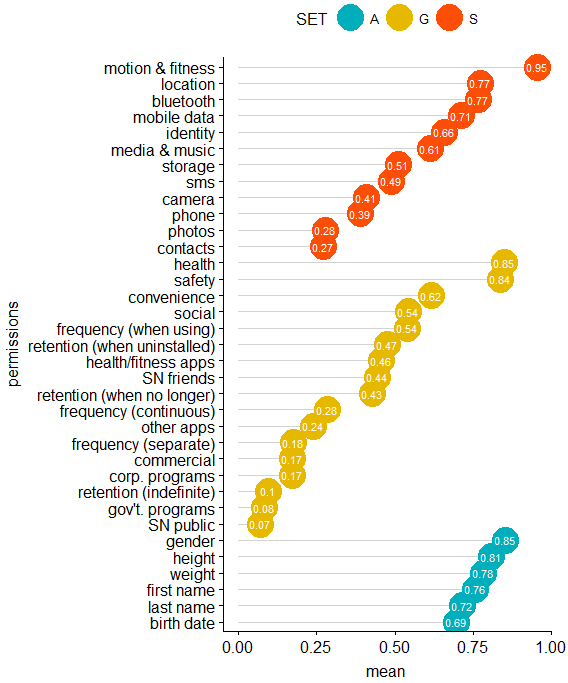
\includegraphics[width=\linewidth]{figures/sum2.png}
	\caption{Average values of each privacy permissions (1-allow, 0-deny).}
	\label{fig:mean}      
\end{figure}
%
%\begin{figure}[ht]
%	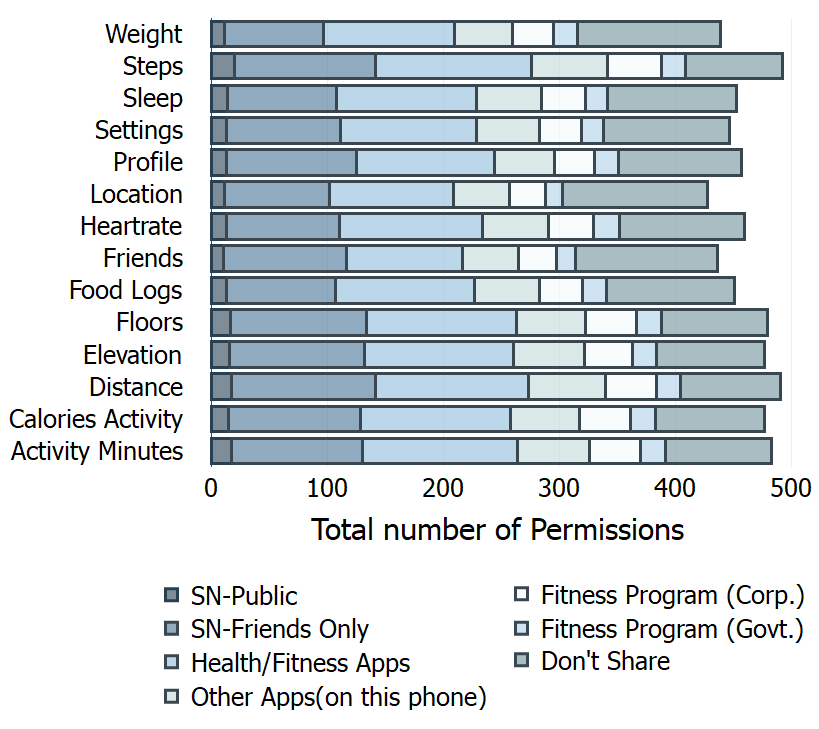
\includegraphics[width=0.98\linewidth]{figures/fdata6.png}
%	\caption{Distribution of fitness data (F set) with respect to different Entity Types (G set).}
%	\label{fig:fdata}      
%\end{figure}

%ODNAN: edited a little to connect F-G entity types
%We do not show the fitness data (F set) in Figure~\ref{fig:mean} because the permissions for these data are requested for multiple entity types of the G set, as discussed in Section~\ref{sec:fset}. Hence, we present these data in Figure~\ref{fig:fdata} instead, showing each permission for each GDPR \textit{EntityType}. 
%%Participants are likely to share their Fitness data (as 40.33\% of the respondents have already shared them in real life scenario). What differs is their perception for the receiving entity of the data. Figure~\ref{fig:fdata} shows the distribution of permissions for different entity types. 
%Users are more likely to give permission to their friends on social networks and to other health/fitness apps, and they are less likely to give permission to share their data with government fitness programs or publicly on social media. As for various data types, steps are shared most openly, while location, friends, and weight are shared less openly.
%
%Upon further inspection, we note that participants tend to share either (almost) all or (almost) none of fitness data with an entity. This suggests that Fitness data permissions are more likely to be influenced by the receiver (``who'') rather than the specific data item (``what'').
%%NEW
%%NEW:ODNAN: i am trying to remind again the reader here that entity type is from G and is split from F 
%As discussed in Section \ref{sec:ppiot}, these ``who'' parameters are instances of the GDPR \textit{EntityType}. Therefore, we expect that clustering F permissions should provide a unanimous deny/share for all items, while clustering G permissions should provide more nuanced clusters of different entity types receiving the data specified in the F set.


\section{Predicting users' Preference (partial original work)}
We predict participants' \textit{allow}/\textit{deny} decision using machine learning methods. Our dataset shows considerable variability between participants' privacy preferences---a finding that is broadly reflected in the privacy literature~\cite{knijnenburg2013dimensionality}. Using clustering, one can capture the preferences of various users with a higher level of accuracy. Hence, the goal of this section is to find a concise set of profiles, clusters, that can represent the variability of the permission settings among our study participants. 

We cluster participants' permissions with Weka\footnote{\url{https://www.cs.waikato.ac.nz/ml/weka/}} using the K-modes clustering algorithm with default settings. The K-modes algorithm follows the same principles as the more common K-means algorithm, but it is more suitable for the nominal variables in our dataset.

%Privacy-setting Profiles are then generated from each cluster. The advantage of this method is that users can set up all their privacy settings by one or few clicks. However, in the other hand, there are some drawbacks about this approach. Advanced users may still need to check each of the settings and change what they need. And the profile provided will be long since all the settings from four different sets are presented in a single profile. Moreover, assume we cluster the users into $n$ clusters, the naive method will only provide $n$ possible profile recommendations to the users. However, if we generate profiles from each of the four datasets (A, F, S, and G), a total number of $n^4$ different combinations of profiles can be recommended, providing a more fine-grained privacy-setting control to the users than the naive method. In the following, we will discuss our method that generates set-based profiles for each of the four datasets, called \textit{sub-profile}.

\begin{figure*}[ht]
	\centering
	\begin{subfigure}[b]{0.4\linewidth}
		\centering
		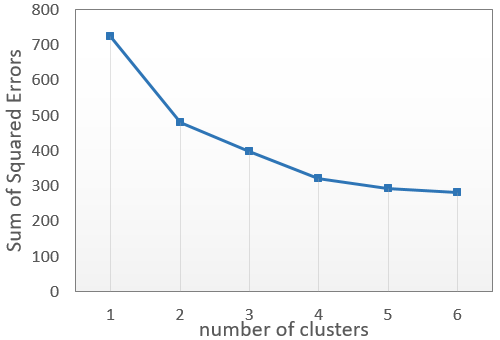
\includegraphics[width=150pt]{figures/Scluster_new4.png}
		\caption{S dataset}
		\label{fig:numS}
	\end{subfigure}
	\begin{subfigure}[b]{0.4\linewidth}
		\centering
		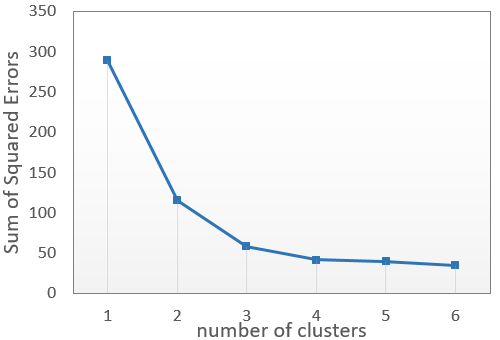
\includegraphics[width=150pt]{figures/Acluster_new4.png}
		\caption{A dataset}
		\label{fig:numA}
	\end{subfigure}
	\begin{subfigure}[b]{0.4\linewidth}
		\centering
		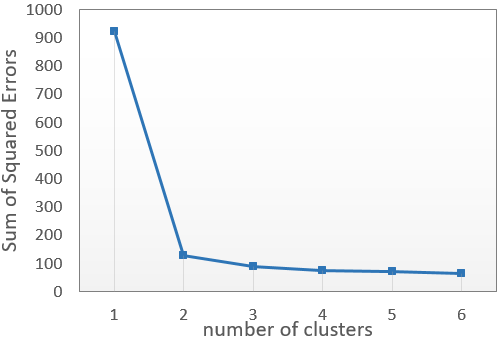
\includegraphics[width=150pt]{figures/Fcluster_new4.png}
		\caption{F dataset}
		\label{fig:numF}
	\end{subfigure}
	\begin{subfigure}[b]{0.4\linewidth}
		\centering
		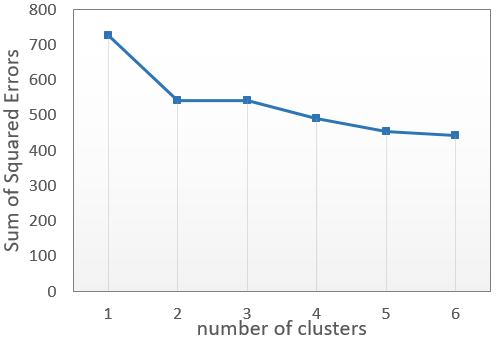
\includegraphics[width=150pt]{figures/Gcluster_new4.png}
		\caption{G dataset}
		\label{fig:numG}
	\end{subfigure}
	\caption{Evaluation of different numbers of clusters for each set.}
	\label{fig:cluster_evaluation}
\end{figure*}


\subsection{Overall Prediction}
In our first clustering attempt we tried to find a set of profiles by clustering the full dataset, including the A, F, S, and G subsets.
A drawback of this method is that, assume we cluster the users into $n$ clusters, this  method will  only provide $n$ possible profiles to be used for recommendations to the users. A further drawback of clustering based on the full set of 45 permissions is that it has high error rates (e.g., the sum of squared error for the viable 4-cluster solution is 1435 and 1688 for 2-cluster solution). In addition, the profile provided will be complicated since all the settings from four different sets are presented in a single profile, making it difficult to explain to the users.

If we instead generate a separate set of $n$ ``subprofiles'' for each of the four datasets (A, F, S, and G), $n^4$  different combinations of profiles can be used for recommendation, providing finer-grained privacy-setting controls to the users compared to clustering the full set. In addition, error rates are lower when clustering each set separately, as shown in Figure \ref{fig:cluster_evaluation}. For example, with only 2 clusters per set, the sum of squared error reduces to 1277 (a 24.3\% reduction). %BART: please enter this number %ODNAN: 1277 is the total sum of the S F A G sum of squared error
An additional benefit is that the profiles for each set can be investigated in more detail. 


%new addition: as suggested by Prof. Bart
In our dataset the fitness data permissions (F set) are specified repeatedly for each Entity Type (part of the G set). We tried to cluster these combinations, taking into account all 98 features (i.e., 14 fitness data per 7 entity types). This analysis resulted in two profiles: one that had ``allow all'' for health and SN public entities (and ``deny all'' for all other entities), and one that had``deny all'' for all entities. This means that: a) very similar results can be obtained by considering the fitness data permissions separately from the Entity Type, and b) as expected, the ``who'' parameter (Entity Type) is more important than the ``what'' parameter (fitness data permissions). 

In the following, we will discuss our method that generates subprofiles for each of the four datasets.


\subsection{2-Cluster Solution}

We first investigate the optimal number of clusters by running the K-modes algorithm for 1-6 clusters with a 70/30 train/test ratio, using the sum of squared errors of the test set for evaluation. The results are shown in Figure~\ref{fig:cluster_evaluation}. Using the elbow method~\cite{kodinariya2013review}, we conclude that 2 is the optimal number of clusters for each dataset\footnote{We obtain similar results using other clustering algorithms, such as Hierarchical Clustering.}. 
%More importantly, the F set shows a distinctive 2-cluster solution as shown in Figure~\ref{figures/fig:fgraph}, which is consistent to the reasons mentioned on Section~\ref{sec:analysis} about the requesting entity type. It is also consistent with the results in~\cite{lee2017privacy}, where the identity of the information requester (\textit{who} context) is an important determinant of people’s privacy decisions, thus in turn results in unanimous allow or deny for the fitness data permissions.
%BART: didn't you split this data by recipient type?



The final cluster centroids of the 2-cluster solution for each dataset are shown in Figure~\ref{fig:privacy_profiles}, together with the results of the 1-cluster solution. %BART: to avoid confusion, we should not call this "full data" but rather "single cluster" %ODNAN: OK
We describe the subprofiles of each set in the subsections below.

%BART: Should we provide accuracies here?
%there is no accuracy yet, instead, the error rates of the clusters which are already in the Figure 7, these are their respective centroid
\begin{figure}
	\centering
	\begin{subfigure}[b]{0.4\linewidth}
		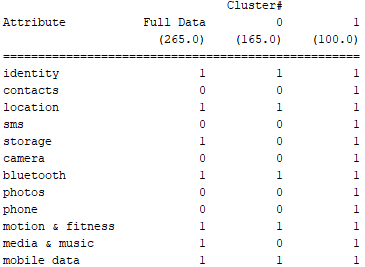
\includegraphics[width=0.85\linewidth]{figures/S_new2.png}
		\caption{S dataset}
		\label{fig:scluster}
	\end{subfigure}
	\begin{subfigure}[b]{0.4\linewidth}
		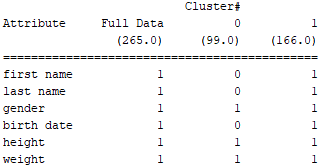
\includegraphics[width=0.85\linewidth]{figures/A_new2.png}
		\caption{A dataset}
		\label{fig:acluster}
	\end{subfigure}
	\begin{subfigure}[b]{0.4\linewidth}
		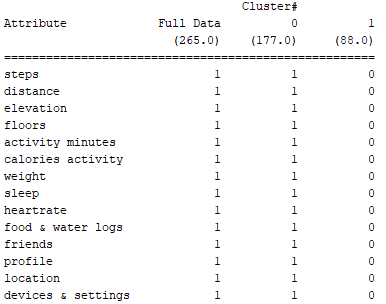
\includegraphics[width=0.85\linewidth]{figures/F_new2.png}
		\caption{F dataset}
		\label{fig:fcluster}
	\end{subfigure}
	\begin{subfigure}[b]{0.4\linewidth}
		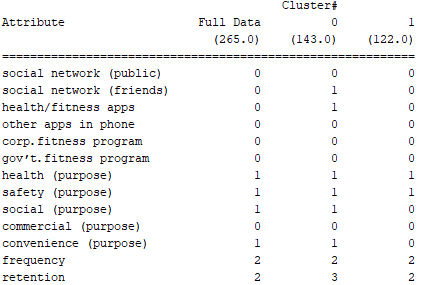
\includegraphics[width=0.85\linewidth]{figures/G_new2.png}
		\caption{G dataset}
		\label{fig:gcluster}
	\end{subfigure} 
	\caption{Privacy profiles from the two clustering methods:  1-cluster results (full data) and 2-clusters results (privacy subprofiles)  for each dataset(allow=1, deny=0, except for frequency \& retention)}
	\label{fig:privacy_profiles}
\end{figure}


\subsubsection{The \textit{S} Set}
\begin{itemize}
	\item \textbf{Minimal} (cluster 0): this subprofile allows the minimum permissions needed to effectively run a fitness app. This includes identity, location, bluetooth, motion \& fitness, and mobile data permissions.
	
	\item \textbf{Unconcerned} (cluster 1): this subprofile allows all permissions in this dataset.
\end{itemize}

\subsubsection{The \textit{A} Set}
\begin{itemize}
	\item \textbf{Anonymous} (cluster 0): this subprofile shares only users' gender, height and weight information but not their birth date or first and last name.
	
	\item \textbf{Unconcerned} (cluster 1): this subprofile shares all data requested in this dataset.
\end{itemize}

\subsubsection{The \textit{F} Set}
\begin{itemize}
	\item \textbf{Unconcerned} (cluster 0): this subprofile shares all fitness data with third parties.
	
	\item \textbf{Strict} (cluster 1): this subprofile does not share any fitness data with third parties.
\end{itemize}

%The unanimous deny/allow permission behavior of F set is consistent with the reason provided on Section~\ref{sec:analysis} regarding the effect of the requesting entity type.
%BART: this just calls attention to the fact that you didn't split this data by recipient type...

\subsubsection{The \textit{G} Set}
\begin{itemize}
	\item \textbf{Socially-active} (cluster 0): this subprofile shares data with health/fitness apps and social network friends, but not with other recipients. %BART: Again, shouldn't the recipient be part of the F-set rather than the G-set? This is very confusing!! 
	%ODNAN:the explanation why entity type is for the G set is explained in the GDPR section, moreover, GDPR permissions are not yet part of today's scenario, and that is also true for the entity type 
	%ODNAN: ALready resolved on the email thread
	Sharing is allowed for health, safety, and social purposes but not for commercial purposes.
	
	\item \textbf{Health-focused} (cluster 1): this subprofile does not allow sharing with any third parties. Sharing is allowed only for health and safety purposes. 
\end{itemize}

\section{Profile Prediction (partial original work)}
\label{sec:prediction}


Now that we have identified two privacy ``subprofiles'' per dataset, the next step is to find predictors for the profiles and predict which subprofiles each participant belongs to.  

Recommender systems usually ask users to evaluate a few items before giving recommendations regarding all remaining items. Likewise, in our system, we might be able to identify certain permission items inside each privacy subprofile that---when answered by the user---could drive the prediction. Since the items are the permission preferences included in the subprofiles, we define this as the ``direct predicition'' approach.

Additionally, we also explored whether the items from our questionnaire could drive the predicition. Since these items are not part of the privacy subprofiles, we define this as the ``indirect prediction'' approach. For each approach and for each subset of data (S, A, F, and G sets), we develop decision trees that will enable us to predict which subprofile best describes a user. The trees contain the subprofile items (direct prediction) or questionnaire items (indirect prediction) that can be asked to classify each user into their correct subprofile.

We developed our decision trees using the J48 decision tree learning algorithm and evaluated the resulting decision tree using cross validation.%J48 is an efficient and widely used decision tree algorithm that can be used for classification~\cite{patil2013performance}. Previous work shows the effectiveness of this approach to predict privacy settings within each cluster~\cite{bahirat2018data}; here we take the opposite approach and use it to predict cluster assignments instead. In our approach, the J48 algorithm extracts the permission items (for the direct prediction) or questionnaire items (for the indirect prediction) that classify a new user into the correct subprofile with the highest possible accuracy.

%The evaluation of all developed J48 trees was performed using k-fold cross validation. %\cite{kohavi1995study}. 


% will we include all the cross-validation results?
%The full details of the evaluation are shown in the Appendix~\ref{sec:appendix}.


\subsection{Direct Prediction Questions}
\label{sec:direct}

In our direct prediction approach, the aim is to ask users to answer certain permission items from each subset as a means to classify them into the correct subprofile (thereby providing a recommendation for the remaining items in that subset). For this approach, we thus classify users using the items in the subset as predictors. 

Our results for this approach are reported in Figure~\ref{fig:tree1}. It shows for each subset the question that best classifies our study participants into the correct subprofile.

\begin{figure}
	\centering
	\begin{subfigure}[b]{0.4\linewidth}
		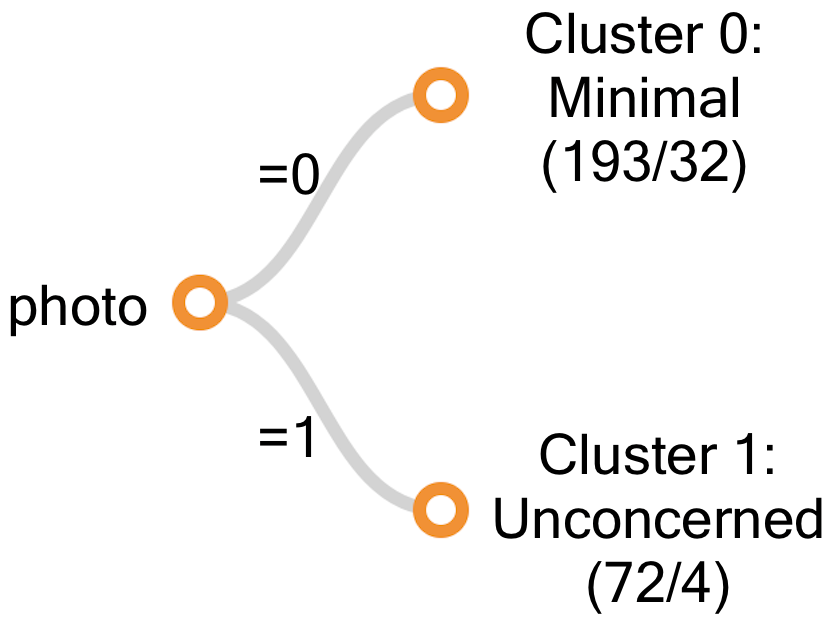
\includegraphics[width=0.5\linewidth]{figures/s_tree1new.png}
		\label{fig:stree1}
		\caption{S set (86.42\%)}
	\end{subfigure}
	\begin{subfigure}[b]{0.4\linewidth}
		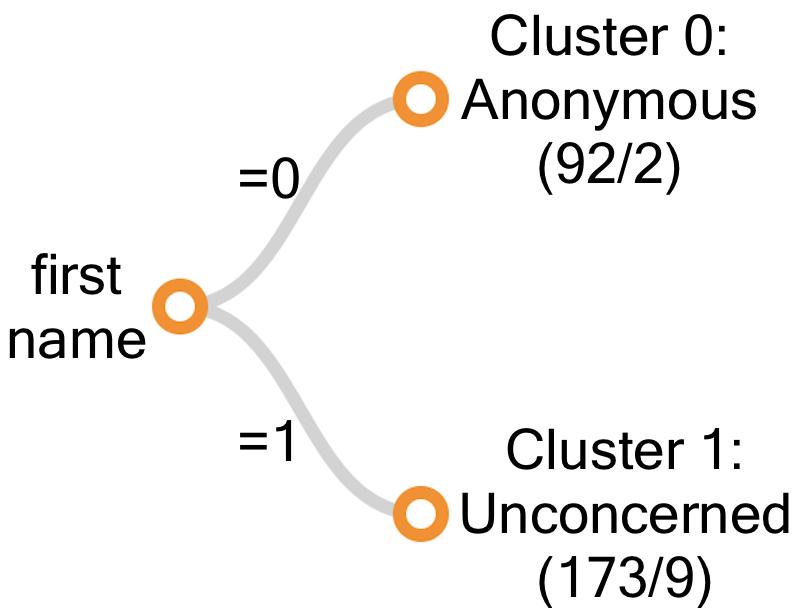
\includegraphics[width=0.5\linewidth]{figures/a_tree1new.png}
		\label{fig:atree1}
		\caption{A set (95.85\%)}
	\end{subfigure}
	\begin{subfigure}[b]{0.4\linewidth}
		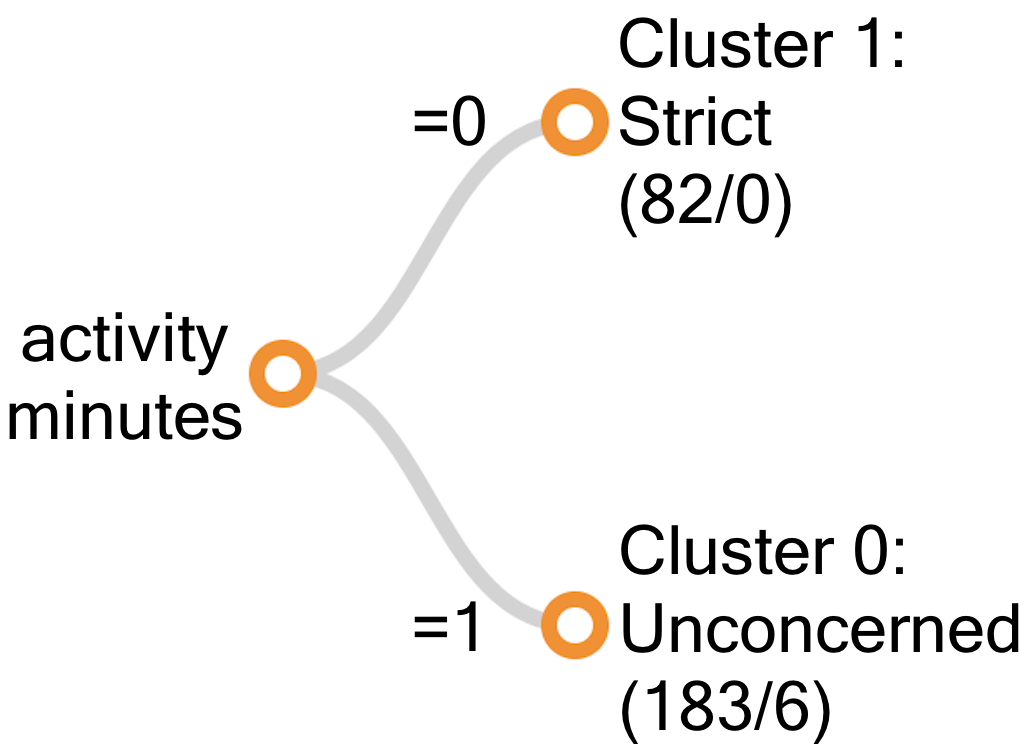
\includegraphics[width=0.5\linewidth]{figures/f_tree1new.png}
		\label{fig:ftree1}
		\caption{F set (97.74\%)}
	\end{subfigure}	
 	\begin{subfigure}[b]{0.4\linewidth}
	 	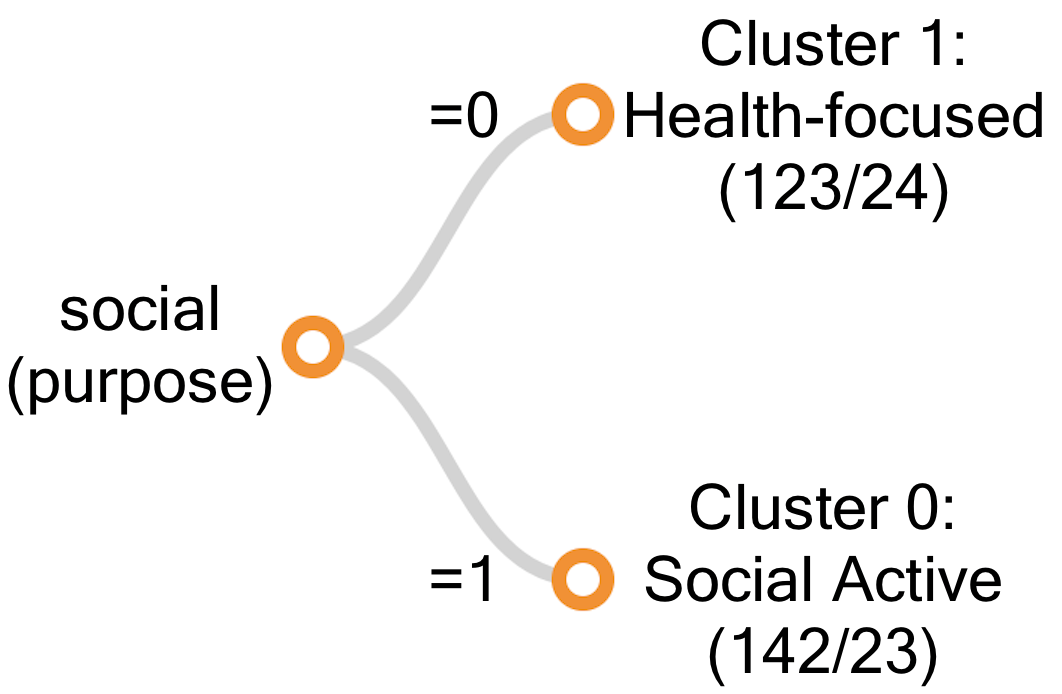
\includegraphics[width=0.5\linewidth]{figures/g_tree1new.png}
	 	\label{fig:gtree1}
	 \caption{G set (82.26\%)}
	\end{subfigure}

	\caption{The permission drivers for the privacy subprofiles and their respective prediction accuracies.}
	\label{fig:tree1}
\end{figure} 


When running tree-based algorithms, a trade-off has to be made between the parsimony and the accuracy of the solution. Parsimony prevents over-fitting and promotes fairness and can be accomplished by pruning the decision trees. In our study, while multi-item trees may provide better predictions, the increase in accuracy is not significant compared to the single-item trees presented in Figure~\ref{fig:tree1}. These single-item solutions already obtained a high accuracy, and their parsimony prevents over-fitting and minimizes the number of questions that will need to be asked to the users in order to provide them accurate recommendations. The resulting solution involves a 4-question input sequence---one question for each subset. 

For the S set, the Photo permission is the best subprofile predictor. This is one of the least-shared permissions (see Figure~\ref{fig:mean}), and 94\% of participants who give this permission are correctly classified into the ``Unconcerned'' subprofile, while 83\% of participants who do not give this permission are correctly classified into the ``Minimal'' subprofile. 

For the A set, First name is the best predictor. Again, 94\% of participants who share their first name are correctly classified into the ``Unconcerned'' subprofile, while 98\% of participants who do not share their first name are correctly classified into the ``Anonymous'' subprofile.

For the F set, Activity minutes permission is the best predictor. This is one of the most-shared permissions. 97\% of participants who give this permission are correctly classified into the ``Unconcerned'' subprofile, while 100\% of participants who do not give this permission are correctly classified into the ``Strict'' subprofile.

Finally, for the G set, the best predictor is whether the participants allows data collection for Social purposes. If so, participants are correctly classified into the ``Socially active'' subprofile with 84\% accuracy, otherwise they are classified into the ``Health-focused'' subprofile with 80\% accuracy.


\subsection{Indirect Prediction Questions}

A similar procedure was applied to the questionnaire data concerning the following categories of user traits: privacy attitude, social behavior, negotiability, exercise tendencies and  user demographics (cf. Table \ref{tab:questionnaire} in Appendix).
As will be shown below, the indirect prediction approach has a lower accuracy than the direct approach presented in Section~\ref{sec:direct}. This is expected since the questionnaire items about user traits have no direct relationship with the permission settings in the privacy profiles.
These results are still interesting, though, since they allow the user to avoid making any specific privacy settings. Moreover, the resulting predictors show interesting semantic relationships with the datasets they predict. We discuss these results in more detail below.

\subsubsection{Privacy Attitudes}

We first attempted to use privacy attitudes as predictors of users' subprofiles. The resulting trees for this indirect prediction are shown in Figure~\ref{fig:tree2}.


\begin{figure}
	\centering
	\begin{subfigure}[b]{0.4\linewidth}
		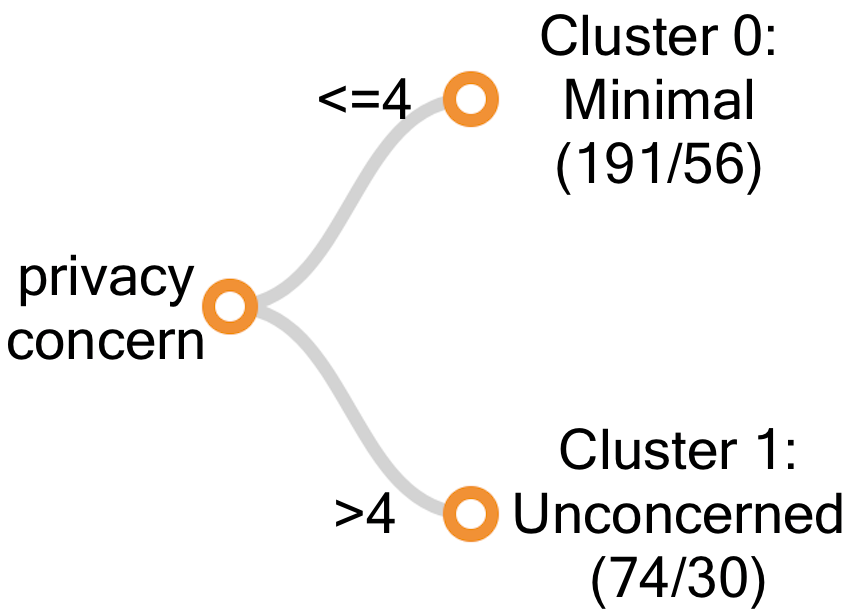
\includegraphics[width=0.5\linewidth]{figures/s_tree2new.png}
		\label{fig:stree2}
		\caption{S set (66.04\%)}
	\end{subfigure}
	\begin{subfigure}[b]{0.4\linewidth}  
		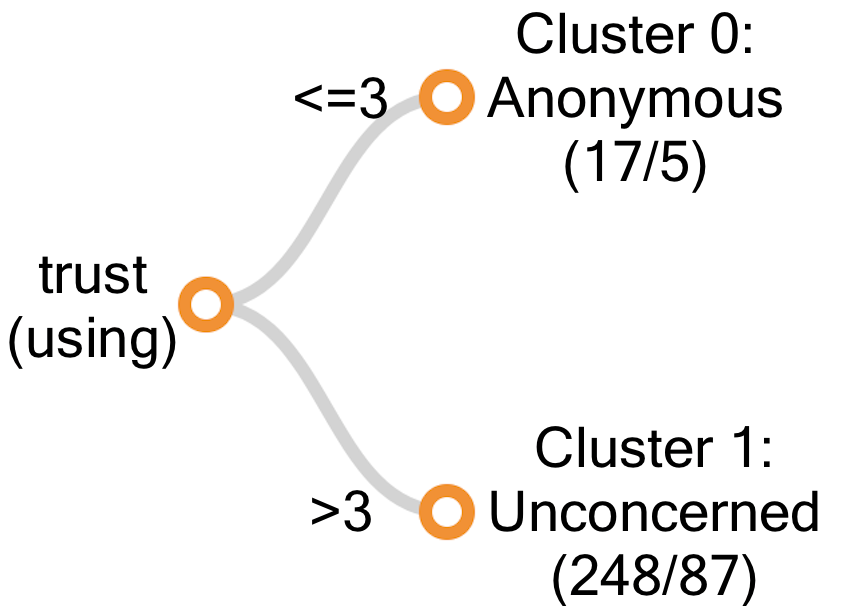
\includegraphics[width=0.5\linewidth]{figures/a_tree2new.png}
		\label{fig:atree2}
		\caption{A set (65.28\%)}
	\end{subfigure}
	\begin{subfigure}[b]{0.4\linewidth} 
		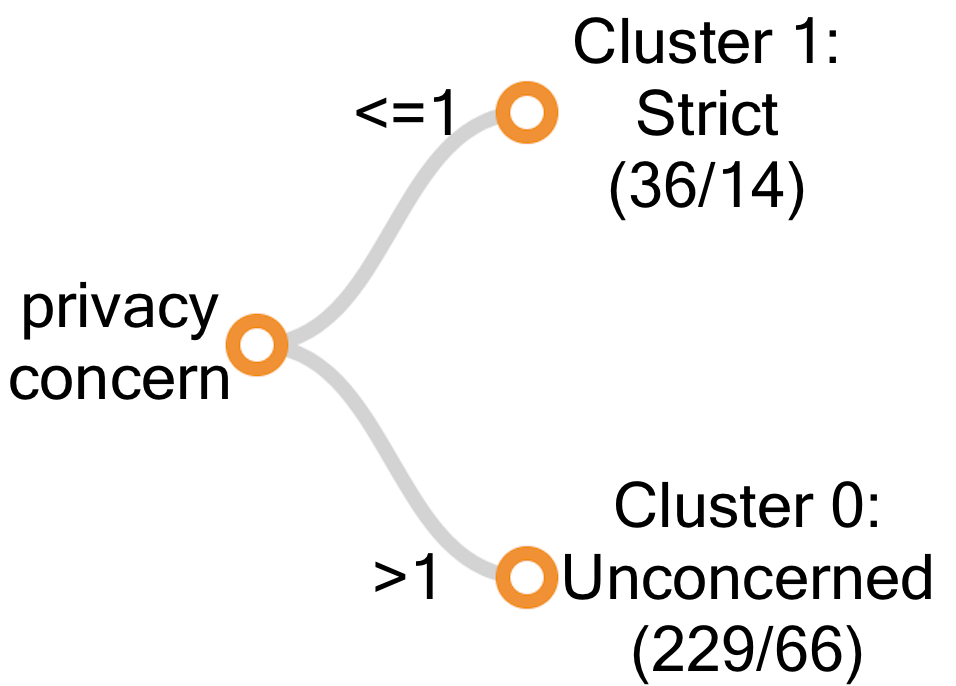
\includegraphics[width=0.5\linewidth]{figures/f_tree2new.png}
		\label{fig:ftree2}
		\caption{F set (69.81\%)}
	\end{subfigure} 
	\begin{subfigure}[b]{0.4\linewidth} 
		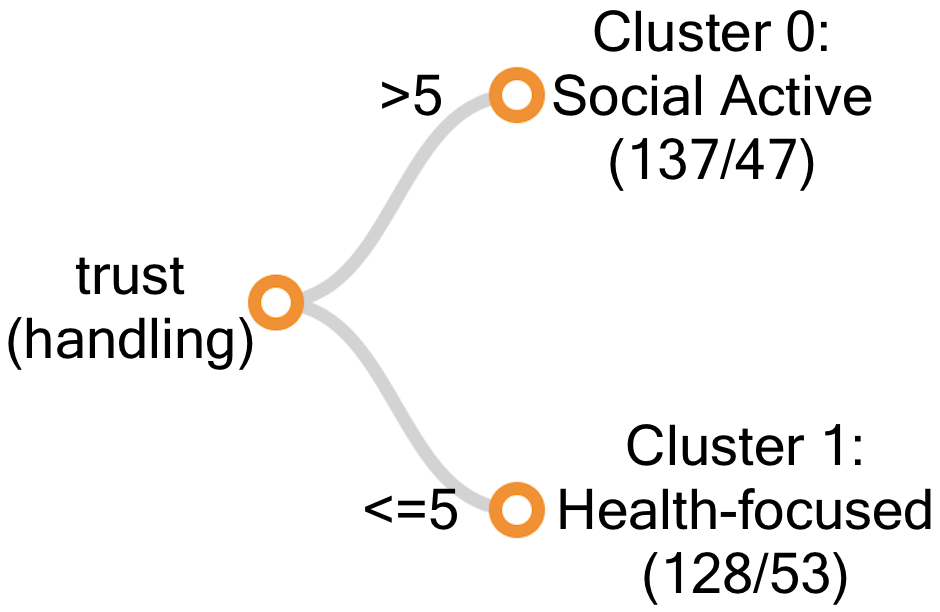
\includegraphics[width=0.5\linewidth]{figures/g_tree2new.png}
		\label{fig:gtree2}
		\caption{G set (62.26\%)}
	\end{subfigure}
	\caption{The attitude drivers for the privacy subprofiles and their respective prediction accuracies.}
	\label{fig:tree2}
\end{figure} 



% TRUST1 question is appropriate for the G Dataset as it is a question on  HANDLING the data.
% I believe the company providing this fitness tracker is trustworthy in handling my information.

%the previous result with hle
% Among the sets, the S set has the most complex solution. It requires users to answer both a healthy living expertise question (``I am able to choose the right healthy-living measures'') and a privacy concern question (``I believe other people are too concerned with online privacy issues''). Both questions are asked on a 7-point scale, and figure~\ref{fig:stree2} shows the complex relationship between users' answers to these two questions and the assigned subprofile. In general, those with lower concerns tend to be in the ``Unconcerned'' subprofile unless they have high expertise, while those who have higher concerns tend to be in the ``Minimal'' subprofile unless they have high expertise. Domain knowledge thus reduces some of the effect of privacy concerns when it comes giving to smartphone permissions to fitness apps.

%new
Among all the privacy attitude questions, ``trust'' and ``privacy concern'' are found to be predicting factors of user subprofiles. Interestingly, there is a single  privacy concern question (``I believe other people are too concerned with online privacy issues'') that predicts the user's S and F subprofiles. Those who agree that people are just too concerned about privacy issues belong to ``Unconcerned'' subprofile, while those who have higher concerns tend to be in the ``Minimal'' subprofile. The same goes for the F set where those who strongly disagree, (1) on a 7pt scale, thinking that it is a major concern belong to the ``Strict'' subprofile. Otherwise they are classified as ``Uncocerned''.
%Domain knowledge thus reduces some of the effect of privacy concerns when it comes giving to smartphone permissions to fitness apps.

%ODNAN:Note, I did an error that I now corrected, it was the privacy concern that solves two sets, not the trust

For the trust question, ``I believe the company is honest when it comes to using the information they provide'', it can be used to predict users' subprofile for the A set. Participants are assigned to the ``Anonymous'' subprofile if they answer this question with ``somewhat disagree'' (3) or below. Those who indicate higher levels of trust are assigned to the ``unconcerned'' subprofile. The A set concerns information provided directly to the fitness app, so it makes sense that trust is a significant predictor of users' willingness to provide such information.

For the G set, those users who agree (6) or extremely agree (7) with the question ``I believe the company providing this fitness tracker is trustworthy in handling my information'' are classified in the ``Socially active'' subprofile, while the remaining users are classified in the ``Health-focused'' subprofile. The question really fits the G set since GDPR permissions are mostly about handling the user information by the third parties. Particularly, it makes sense that users who do not trust the fitness app in handling their information would be assigned to the ``Health-focused'' profile, since this profile prevents the app from sharing their data to any other entity and only allows data collection for the purpose of health and/or safety.

%Those who agree that other people are too concerned with online privacy issues and believe they are able to choose the right healthy-living measures are people who are unconcerned (cluster 1)


The result shows that we managed to capture some semantically relevant relationships between users' attitudes and their assigned privacy profiles. The S and F sets share the same predictor question which makes the final solution a 3-question input sequence that is one less question to the users compared to the direct questions in Section~\ref{sec:direct}.

%ODNAN: changed to SOcial Behavior according to Prof. Ilaria
\subsubsection{Social Behavior}
We also tried to find predictors among the questions about social influence and sociability. The resulting trees for this indirect prediction are shown in Figure~\ref{fig:tree3}.


%\begin{figure}[b]
%	\centering
%	\subfloat[S set (65.66\%)]
%	{  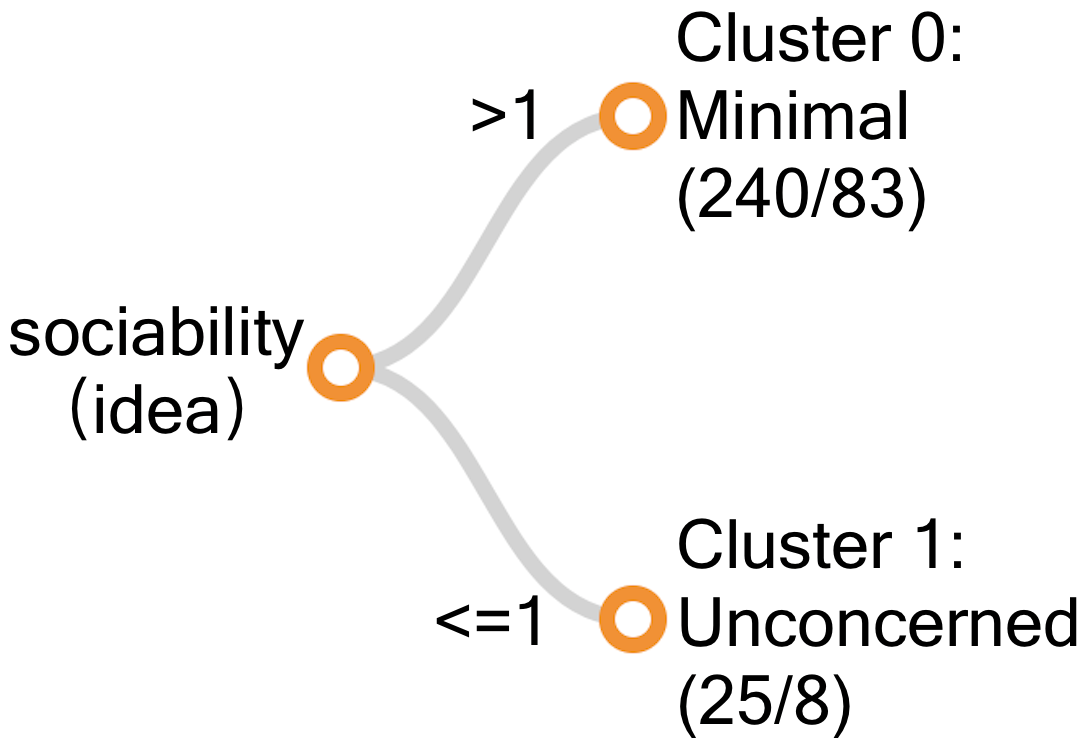
\includegraphics[width=0.5\linewidth]{figures/s_tree3new.png}
%		\label{fig:stree3}}
%	\subfloat[A set (61.89\%)]
%	{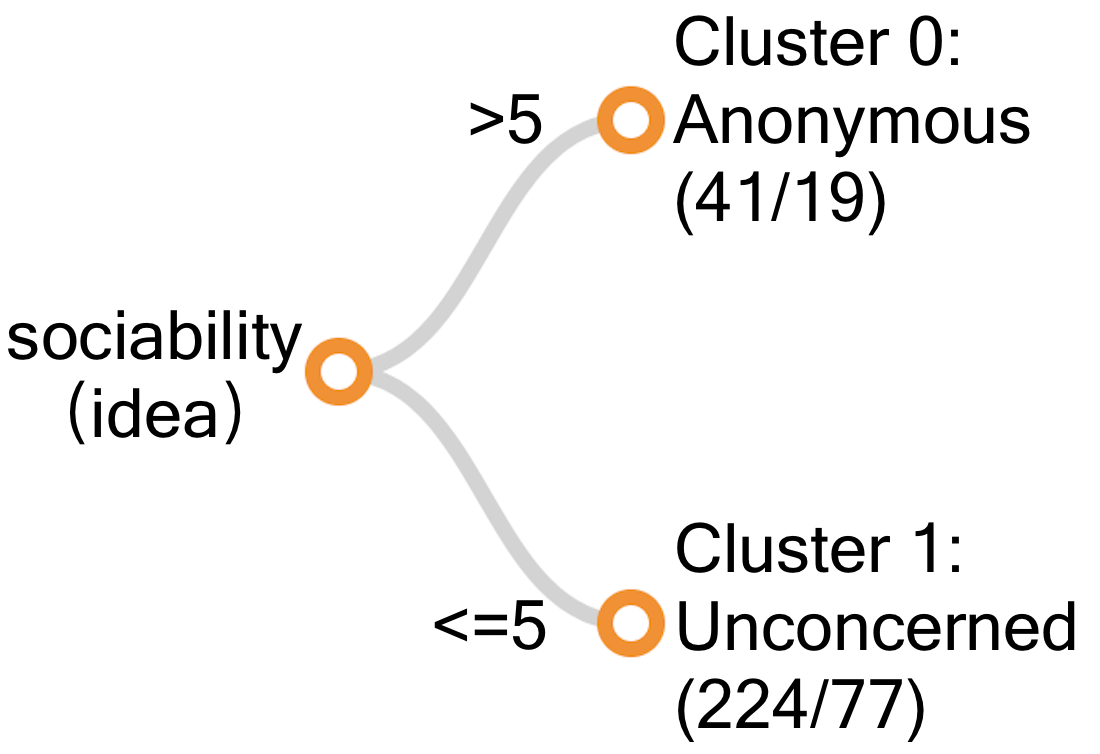
\includegraphics[width=0.5\linewidth]{figures/a_tree3new.png}
%		\label{fig:atree3}}
%	
%	\subfloat[F set (69.43\%)]
%	{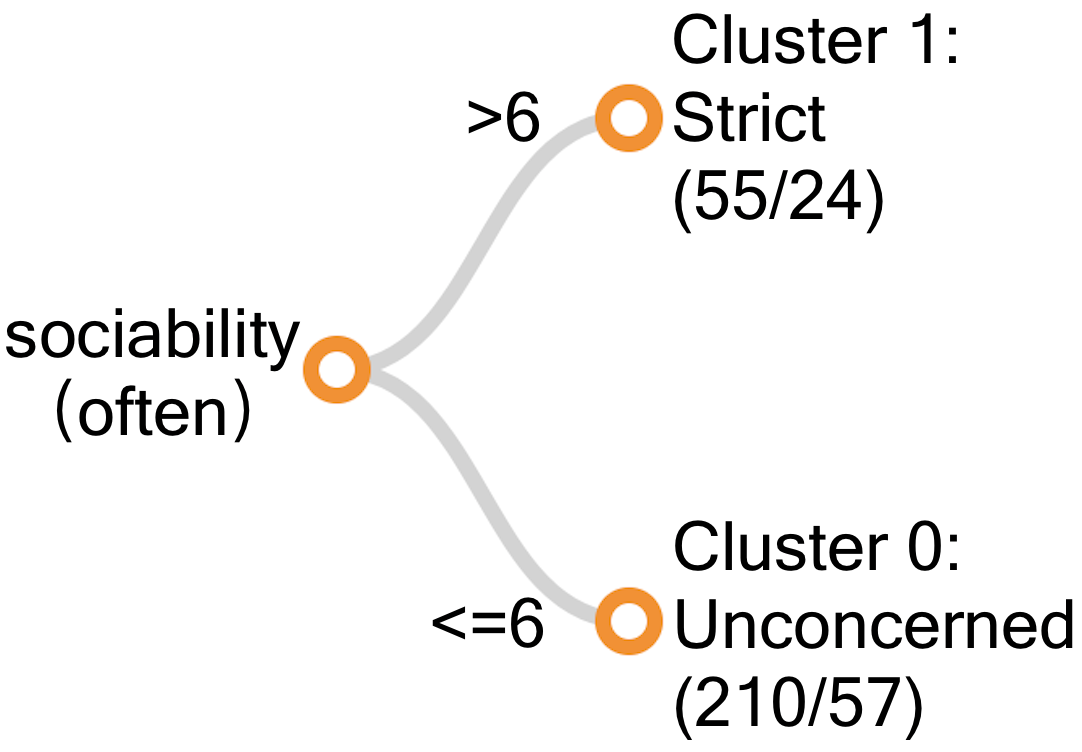
\includegraphics[width=0.5\linewidth]{figures/f_tree3new.png}
%		\label{fig:ftree3}}   
%	\subfloat[G set (61.89\%)]
%	{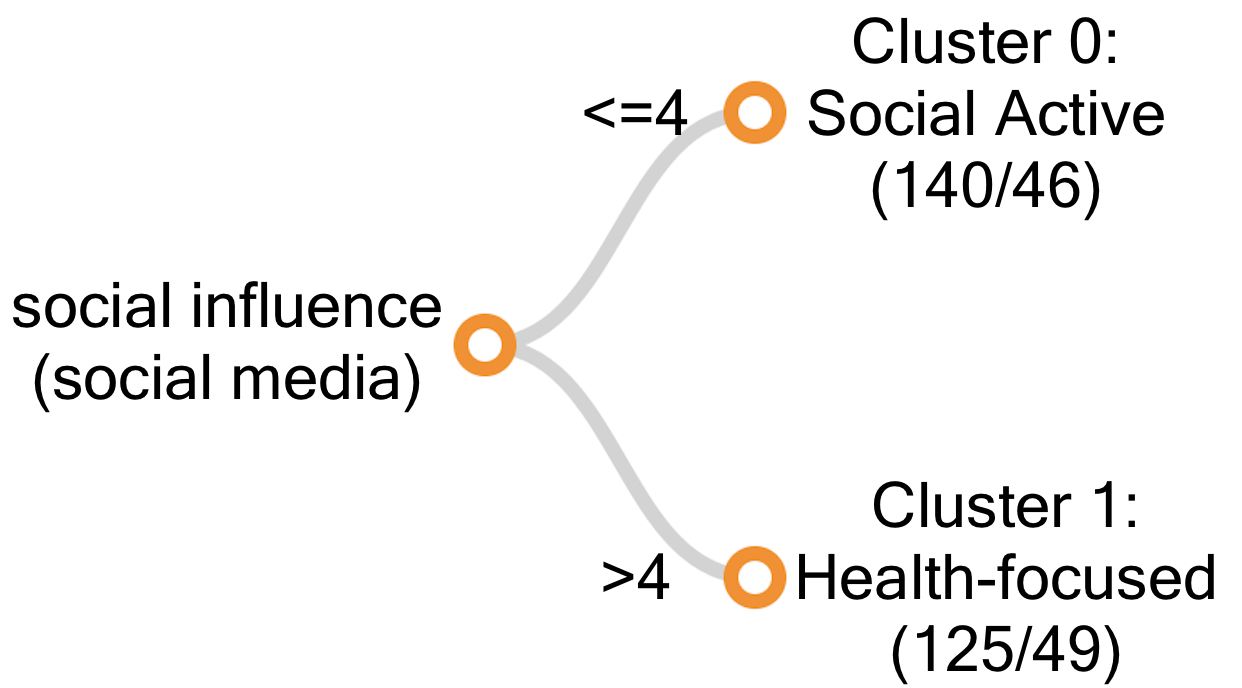
\includegraphics[width=0.5\linewidth]{figures/g_tree3new.png}
%		\label{fig:gtree3}}
%	\caption{The social behavior drivers for the privacy subprofiles and their respective prediction accuracies.}
%	\label{fig:tree3}
%\end{figure} 
\begin{figure}
	\centering
	\begin{subfigure}[b]{0.4\linewidth}
		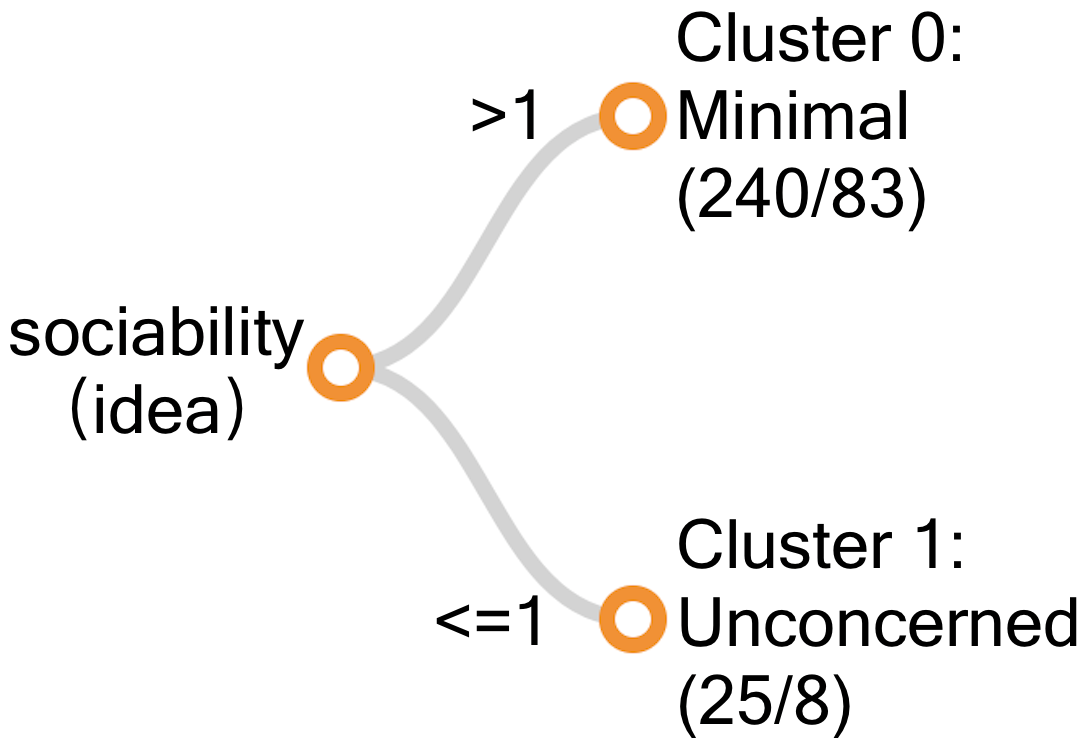
\includegraphics[width=0.5\linewidth]{figures/s_tree3new.png}
		\label{fig:stree3}
		\caption{S set (65.66\%)}
	\end{subfigure}
	\begin{subfigure}[b]{0.4\linewidth}  
		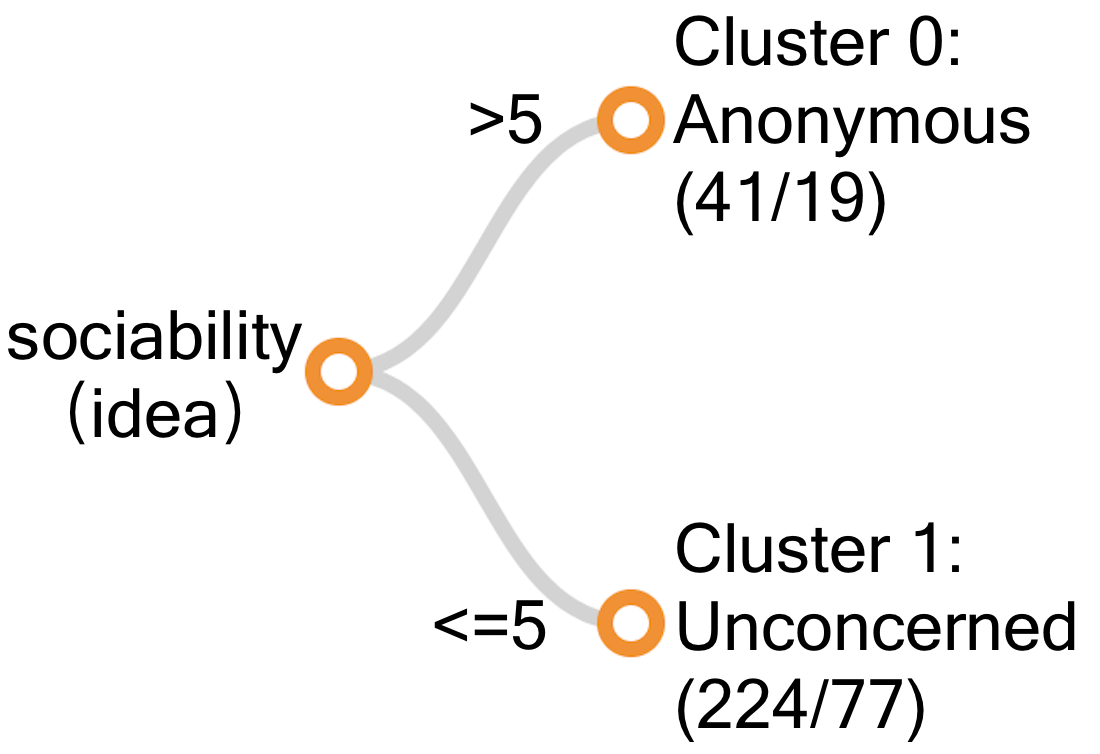
\includegraphics[width=0.5\linewidth]{figures/a_tree3new.png}
		\label{fig:atree3}
		\caption{A set (61.89\%)}
	\end{subfigure}
	\begin{subfigure}[b]{0.4\linewidth} 
		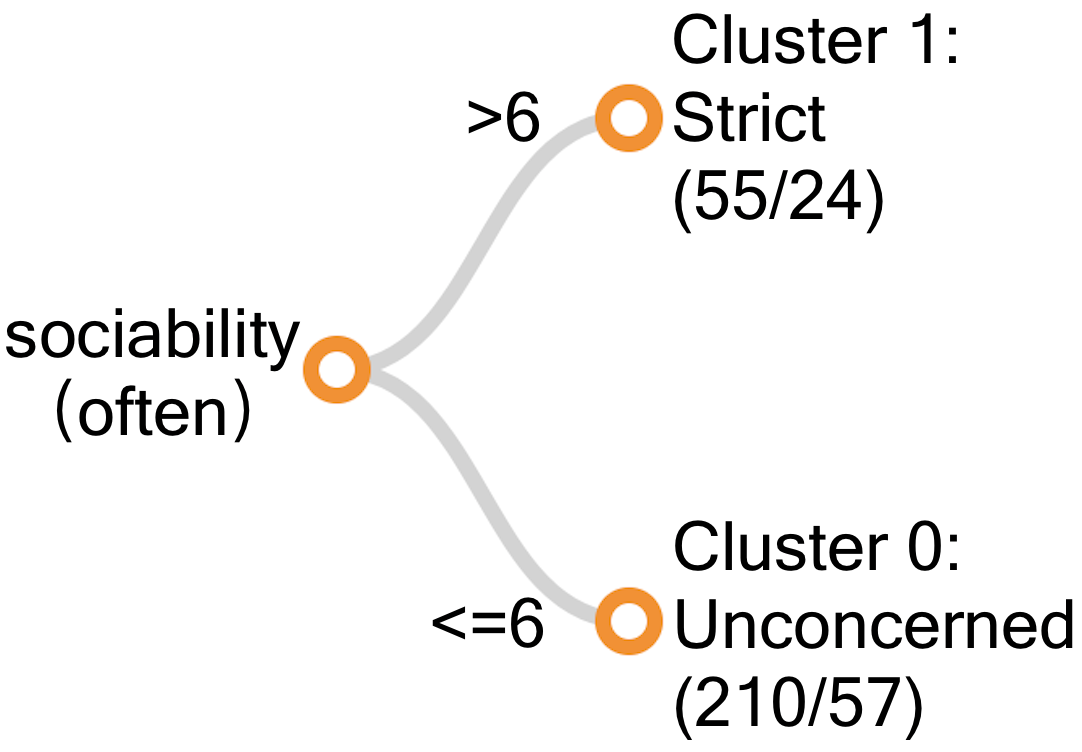
\includegraphics[width=0.5\linewidth]{figures/f_tree3new.png}
		\label{fig:ftree3}
		\caption{F set (69.43\%)}
	\end{subfigure} 
	\begin{subfigure}[b]{0.4\linewidth} 
		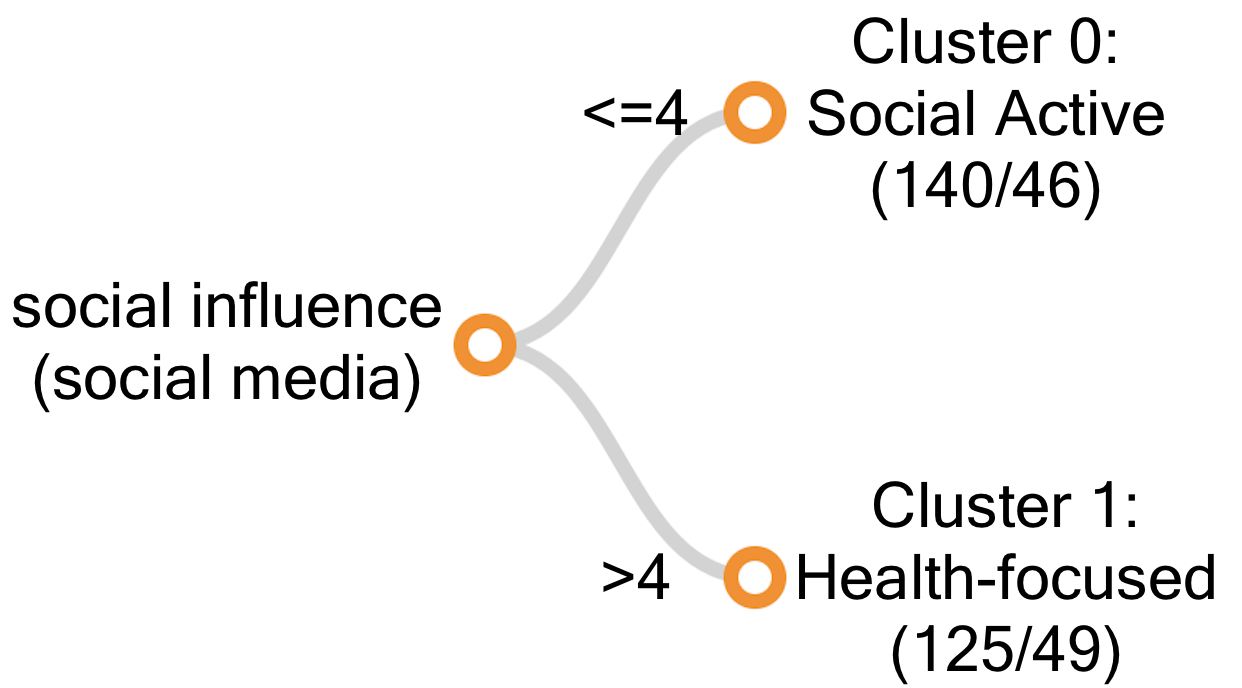
\includegraphics[width=0.5\linewidth]{figures/g_tree3new.png}
		\label{fig:gtree3}
		\caption{G set (61.89\%)}
	\end{subfigure}
	\caption{The social behavior drivers for the privacy subprofiles and their respective prediction accuracies.}
	\label{fig:tree3}
\end{figure}


A single sociability question can be used to predict subprofiles for both the S and A sets. For the S set, users who are completely open (1) to the idea of meeting new friends when they exercise are classified in the ``Unconcerned'' subprofile, otherwise they are classified in the ``Minimal'' subprofile.

For the A set, users who are likely not (6) or definitely not (7) open to meeting new friends are classified in the ``Anonymous'' subprofile, otherwise they are classified in the ``Unconcerned'' subprofile.

For the F set, users who have never (7) met any new friends while exercising are classified into the ``Strict'' subprofile, while others are classified into the ``Unconcerned'' subprofile. This, as well as the findings regarding the S and A sets, seem to suggest that users'  disclosure of personal information is likely to be related with their tendency to socialize while using fitness apps.

For the G set, users who are influenced to do exercise if their social media friends also exercise (i.e., ``definitely yes'' to ``neutral'' (1-4)) are classified into the ``Socially active'' subprofile, otherwise they are classified into the ``Health-focused'' subprofile.

Again, we found interesting semantic relationships between social influence and sociability while exercising and users' privacy-related behaviors: users who are more prone to reap social benefits from exercising are more likely to give the app more widespread permissions. Similar to privacy attitudes, these predictors only involve a 3-question input sequence.


\subsubsection{Negotiability of Privacy Settings}

We also attempted to use the negotiability of users' privacy settings as input for the subprofile prediction. Figure~\ref{fig:tree4} shows the tree-learning solutions for this approach.

%\begin{figure}[b]
%	\centering
%	\subfloat[S set (73.21\%)]
%	{  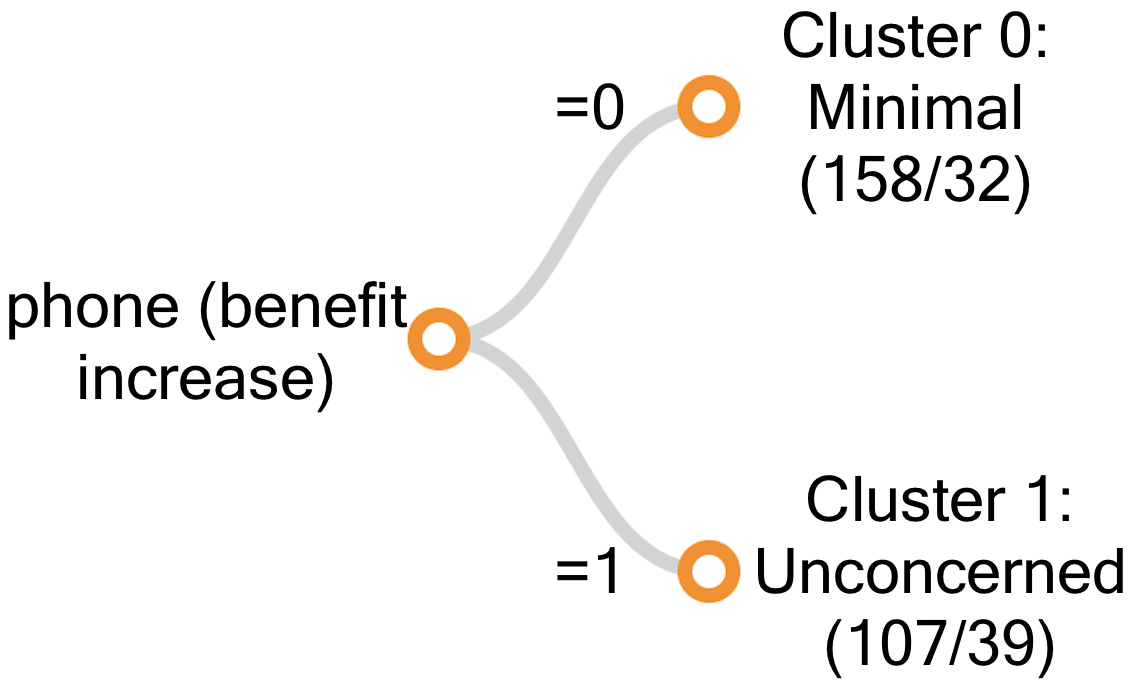
\includegraphics[width=0.5\linewidth]{figures/s_tree4new.png}
%		\label{fig:stree4}}
%	\subfloat[A set (62.26\%)]
%	{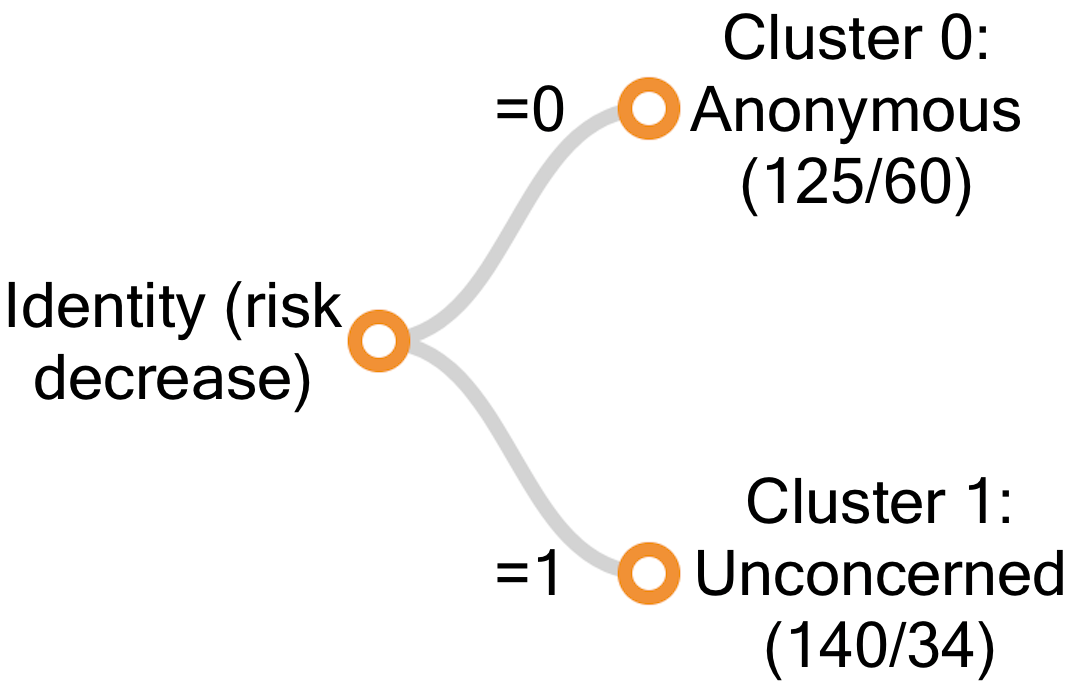
\includegraphics[width=0.5\linewidth]{figures/a_tree4new.png}
%		\label{fig:atree4}}
%	
%	\subfloat[F set (72.08\%)]
%	{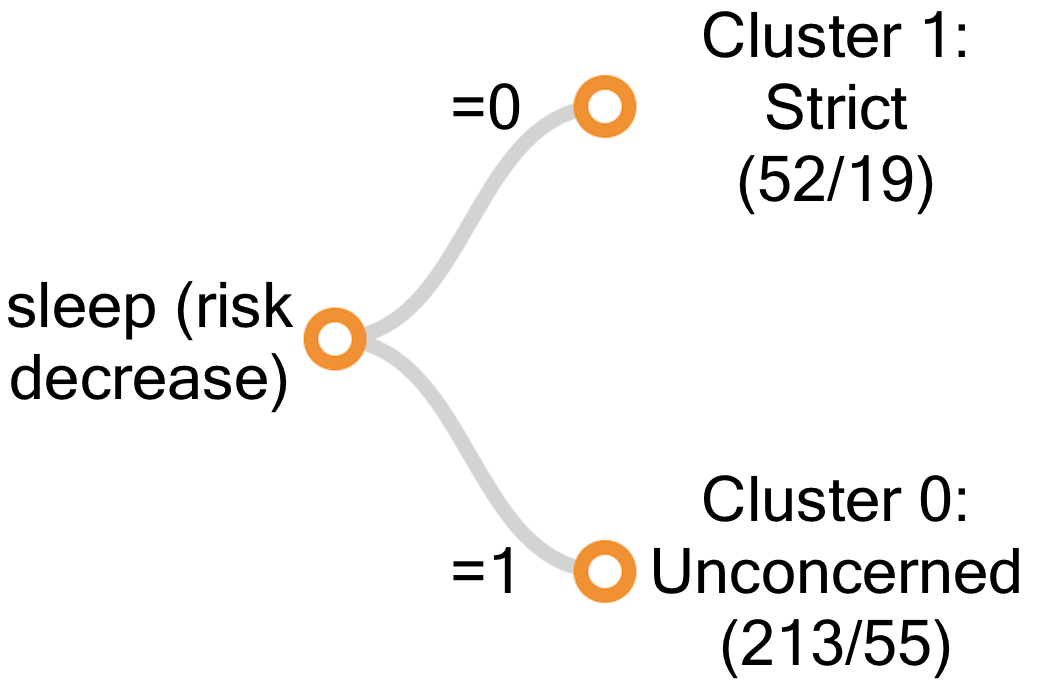
\includegraphics[width=0.5\linewidth]{figures/f_tree4new.png}
%		\label{fig:ftree4}}   
%	\subfloat[G set (66.41\%)]
%	{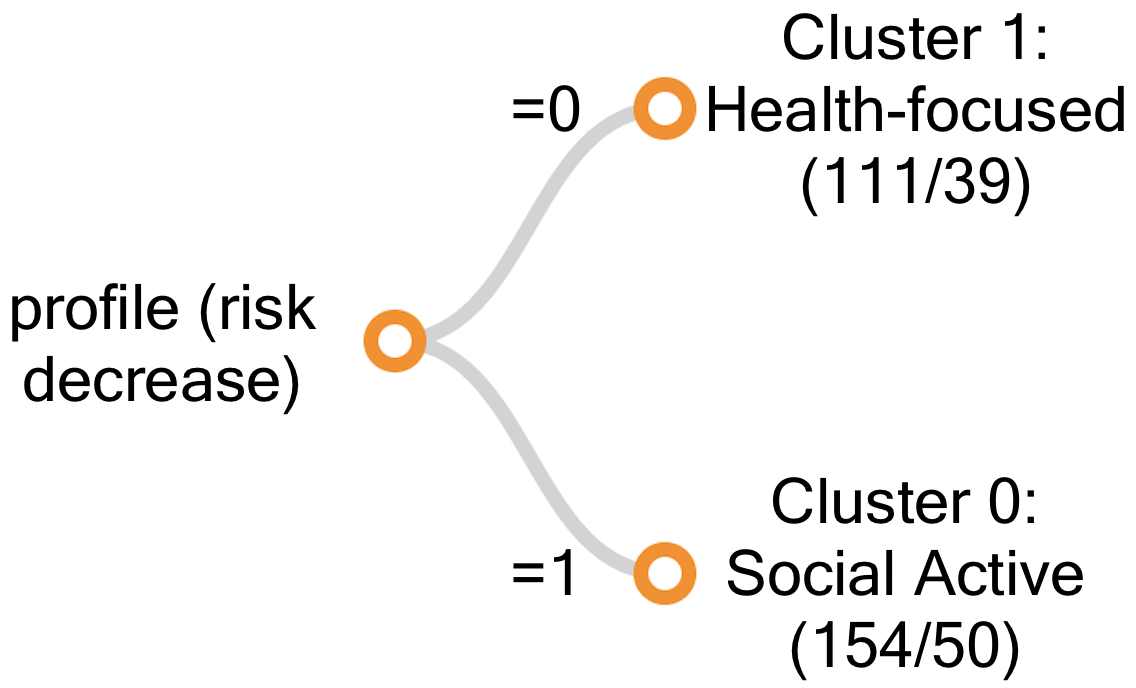
\includegraphics[width=0.5\linewidth]{figures/g_tree4new.png}
%		\label{fig:gtree4}}
%	\caption{The user negotiability drivers for the privacy subprofiles and their respective prediction accuracies.}
%	\label{fig:tree4}
%\end{figure} 
\begin{figure}
	\centering
	\begin{subfigure}[b]{0.4\linewidth}
		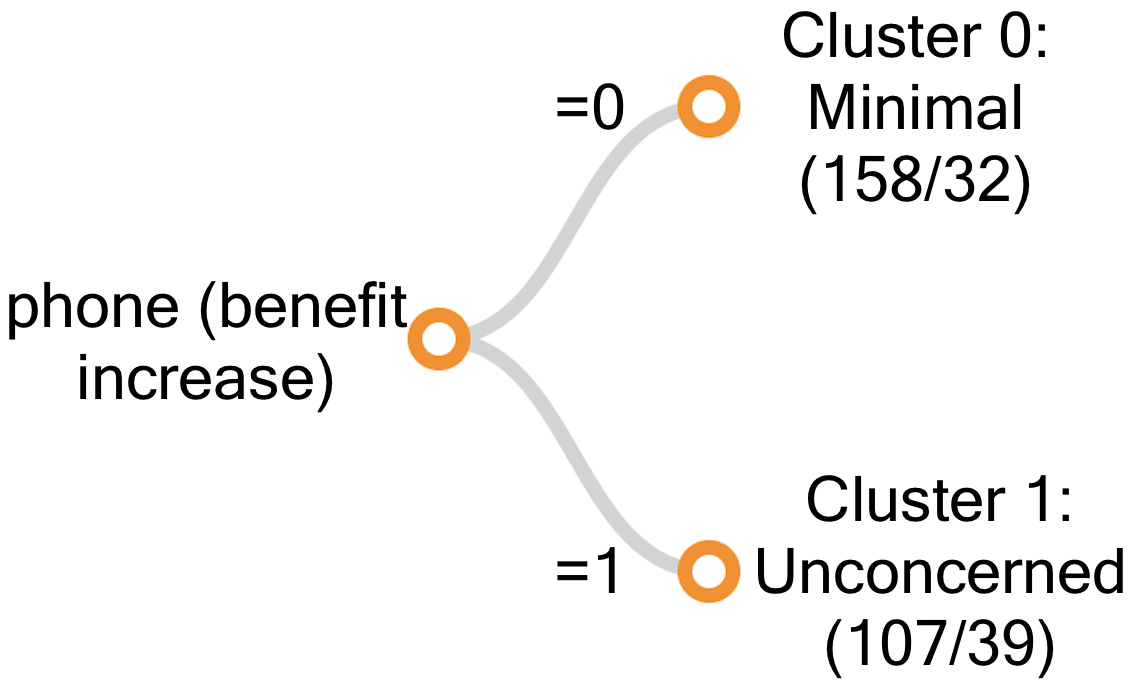
\includegraphics[width=0.5\linewidth]{figures/s_tree4new.png}
		\label{fig:stree4}
		\caption{S set (73.21\%)}
	\end{subfigure}
	\begin{subfigure}[b]{0.4\linewidth}  
		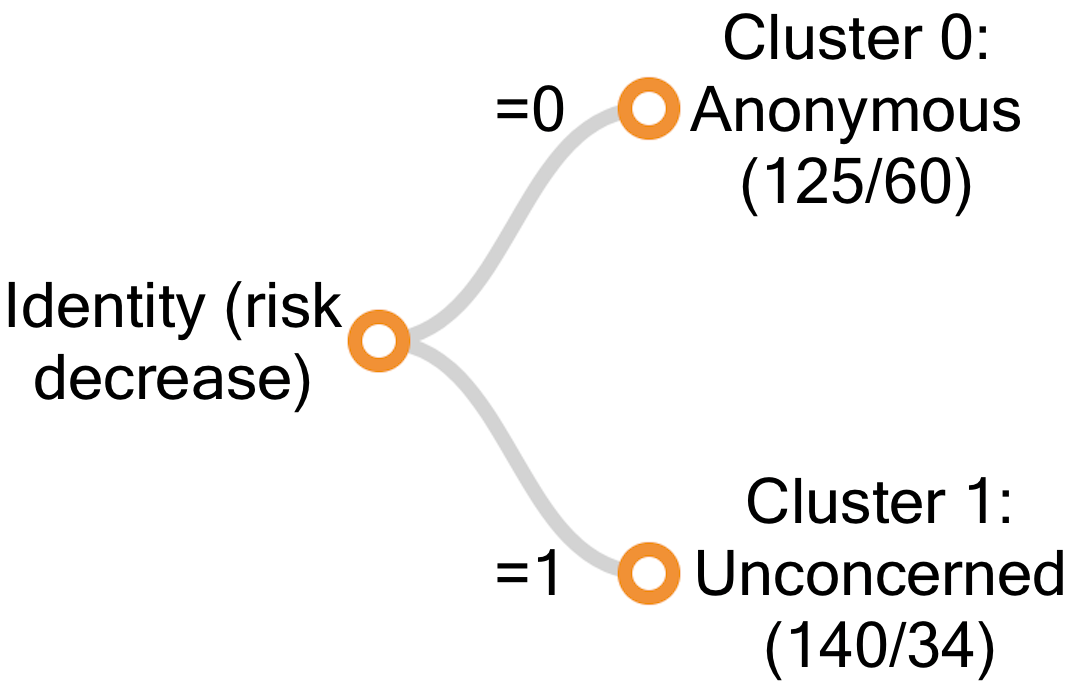
\includegraphics[width=0.5\linewidth]{figures/a_tree4new.png}
		\label{fig:atree4}
		\caption{A set (62.26\%)}
	\end{subfigure}
	\begin{subfigure}[b]{0.4\linewidth} 
		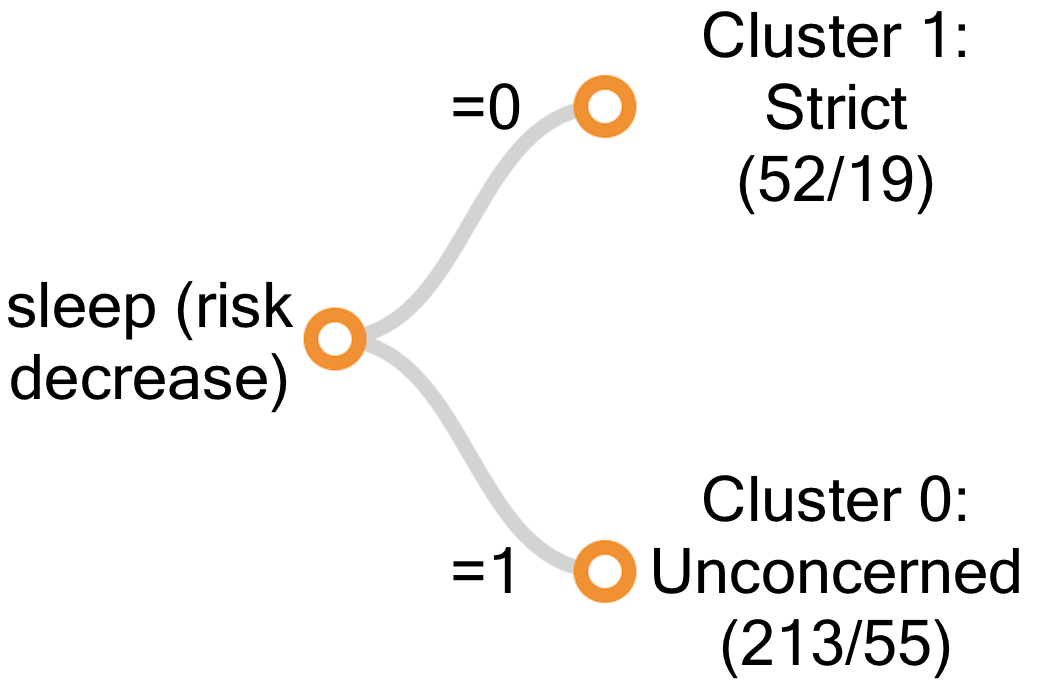
\includegraphics[width=0.5\linewidth]{figures/f_tree4new.png}
		\label{fig:ftree4}
		\caption{F set (72.08\%)}
	\end{subfigure} 
	\begin{subfigure}[b]{0.4\linewidth} 
		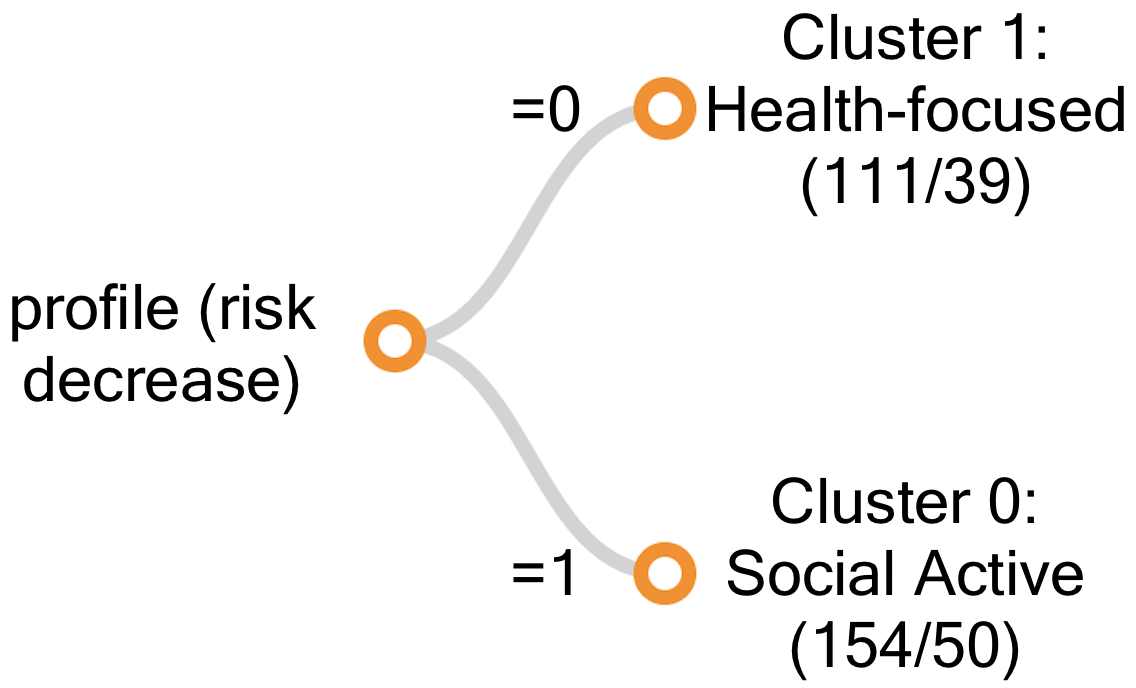
\includegraphics[width=0.5\linewidth]{figures/g_tree4new.png}
		\label{fig:gtree4}
		\caption{G set (66.41\%)}
	\end{subfigure}
	\caption{The user negotiability drivers for the privacy subprofiles and their respective prediction accuracies.}
	\label{fig:tree4}
\end{figure}

For the S set, users who are willing to give the Phone permission (access phone calls and call settings) if the benefits increase are classified into the ``Unconcerned'' subprofile, while users who refuse to share the Phone permission even if the benefits increase are classified into the ``Minimal'' subprofile. In other words, the privacy preferences of the latter group are not negotiable; they will still share only the minimum permissions needed to run the tracker, even if the benefits increase.

For the A set, users who are willing to give the Identity permission (account and/or profile information) if the risks decrease are classified into the ``Unconcerned'' subprofile, otherwise they are classified into the ``Anonymous'' subprofile. Interestingly, the Identity permission is part of the S set rather than the A set, but it semantically coincides with the items in the A set, which include the user's name and birth date (i.e., identifying information). As such, it makes sense that users who are unwilling to share their phone's identifier even when the risks decrease are also unwilling to share their personal identity information.

For the F set, users who share their Sleep fitness data with other third parties if the risks decrease are classified into the ``Unconcerned'' subprofile, otherwise they are classified into the ``Strict'' subprofile. Users in the latter subprofile will not share their fitness data with any other third parties, even if the risk decreases.

For the G set, users who share their fitness app Profile with other third parties if the risks decrease are classified into the ``Socially active'' subprofile, otherwise they are classified into the ``Health-focused'' subprofile. Even though Profile is a permission from the F set, it semantically coincides with the subprofiles of the G set: users in the ``Socially active'' subprofile tend to have permissions that allow them to connect to others while exercising, and sharing one's fitness app Profile is indeed a potential way to connect to other users. As such, it makes sense that users in this subprofile are more willing to share their fitness app Profile if the risks of doing so decrease.
%BONUS: both profile and friends are good identifiers for G set 

The classification accuracy of the negotiability questions is the highest among all ``indirect prediction'' approaches. The most predictive questions also have understandable semantic relationships with the datasets they predict.

\subsubsection{Exercise Tendencies and User Demographics}

%ODNAN:For the exercise questions, the F set do not have a tree formation, but S A and G have, A for exercise_often=60\%, S for hle3=65.66\%, for G only exercise_often=52\% very low! 

We applied J48 learning algorithms to the group of exercise tendency questions and user demographics as well, but we found no significant predictors among these questions. While other studies have found user demographics to be significant predictors of privacy behaviors~\cite{knijnenburg2013helping}, in this particular study we were not able to find any significant predictors among the group of user demographics. 

%User demographics was also found to be weak in providing profiles in the domain of household IoT~\cite{bahirat2018data}.


\subsection{Tree Evaluation}

Figure~\ref{fig:treermse} shows the root mean square error of all the trees produced by the J48 classifier. The evaluation has been executed with $k$-fold cross validation with $k=10$.

\begin{figure}[ht]
	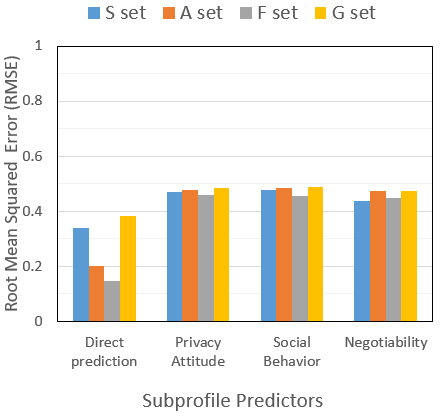
\includegraphics[width=1\linewidth]{figures/rmse4.png}
	\caption{Tree evaluation. Root mean square error for each J48 tree algorithm.}
	\label{fig:treermse}      
\end{figure}

As expected, the ``direct prediction'' approach results in lower error rates than the various ``indirect prediction'' approaches, since in the former approach the items are a direct part of the privacy settings that constitute the subprofiles. Among the ``indirect prediction'' approaches, the \textit{negotiability of privacy settings} has slightly lower error rates. This is not surprising, since it is at least partially related to the privacy settings (yet evaluates whether those settings will change under certain conditions). The prediction accuracies of each tree are reported on the branches in their respective figures (Figure~\ref{fig:tree1} to~\ref{fig:tree4}), and take the form of (\# assigned / \# incorrect). 

\section{Privacy-setting Recommendations (partial original work)}
In this section, we describe different types of guided privacy-setting approaches for fitness Iot users that are based on the previous clustering and machine learning results. 

\subsection{Manual Setting}
\label{sec:manual}

The baseline privacy settings interface is one where users have to manually set their settings (see Figure \ref{fig:manual}). If users do this correctly these manual settings should match their privacy preferences 100\%. However, the process of manually setting one's privacy settings can be very burdensome for the user; our system has a total of 45 permissions that are required to be managed. Under such burden, users are likely going to make mistakes~\cite{madejski2012study}, so the 100\% accuracy may not be achieved through manual settings.

\begin{figure}
	\centering
	\begin{subfigure}[b]{0.24\textheight}
		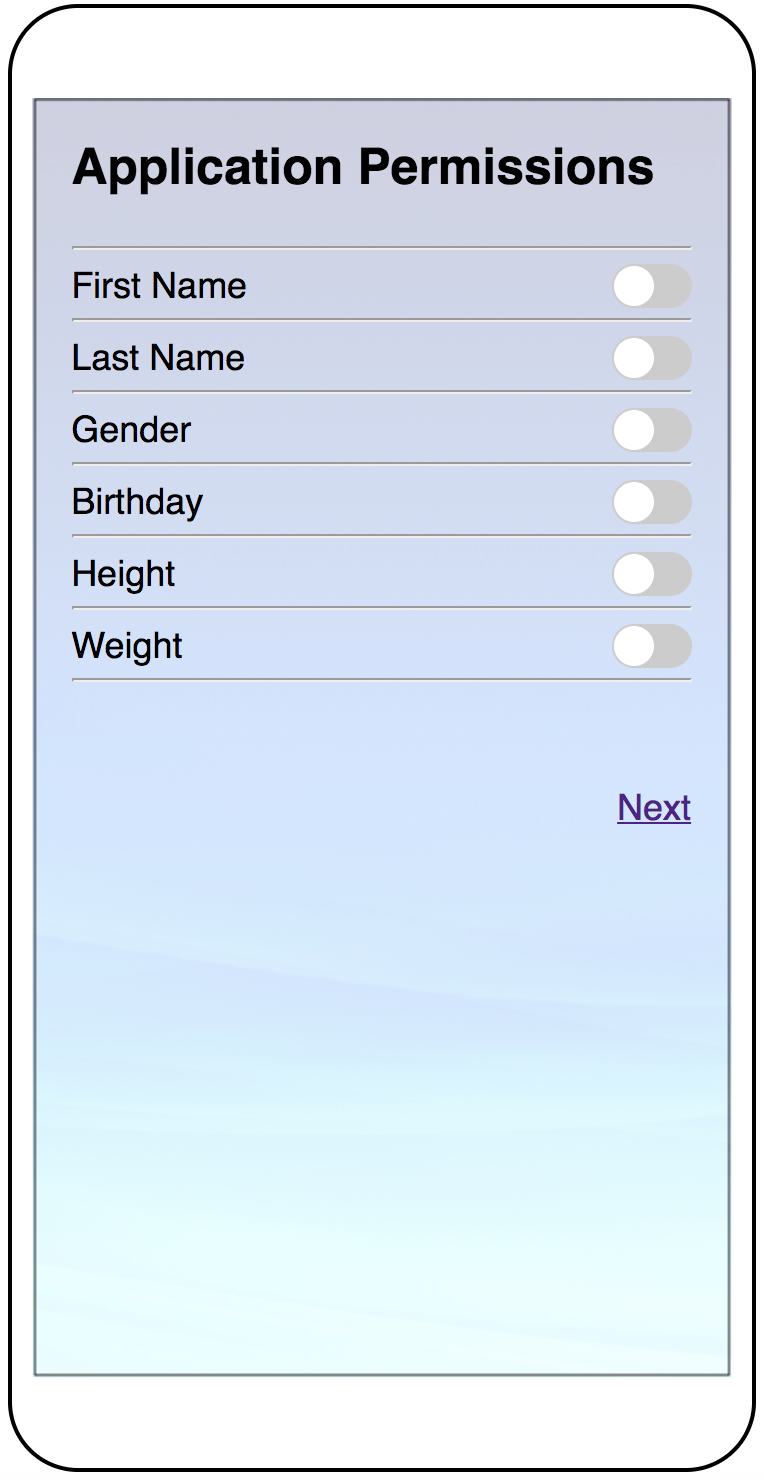
\includegraphics[width=0.24\textheight]{figures/manual1.png}
		\label{fig:manuala}
		\caption{A set}
	\end{subfigure}
	\begin{subfigure}[b]{0.24\textheight}
		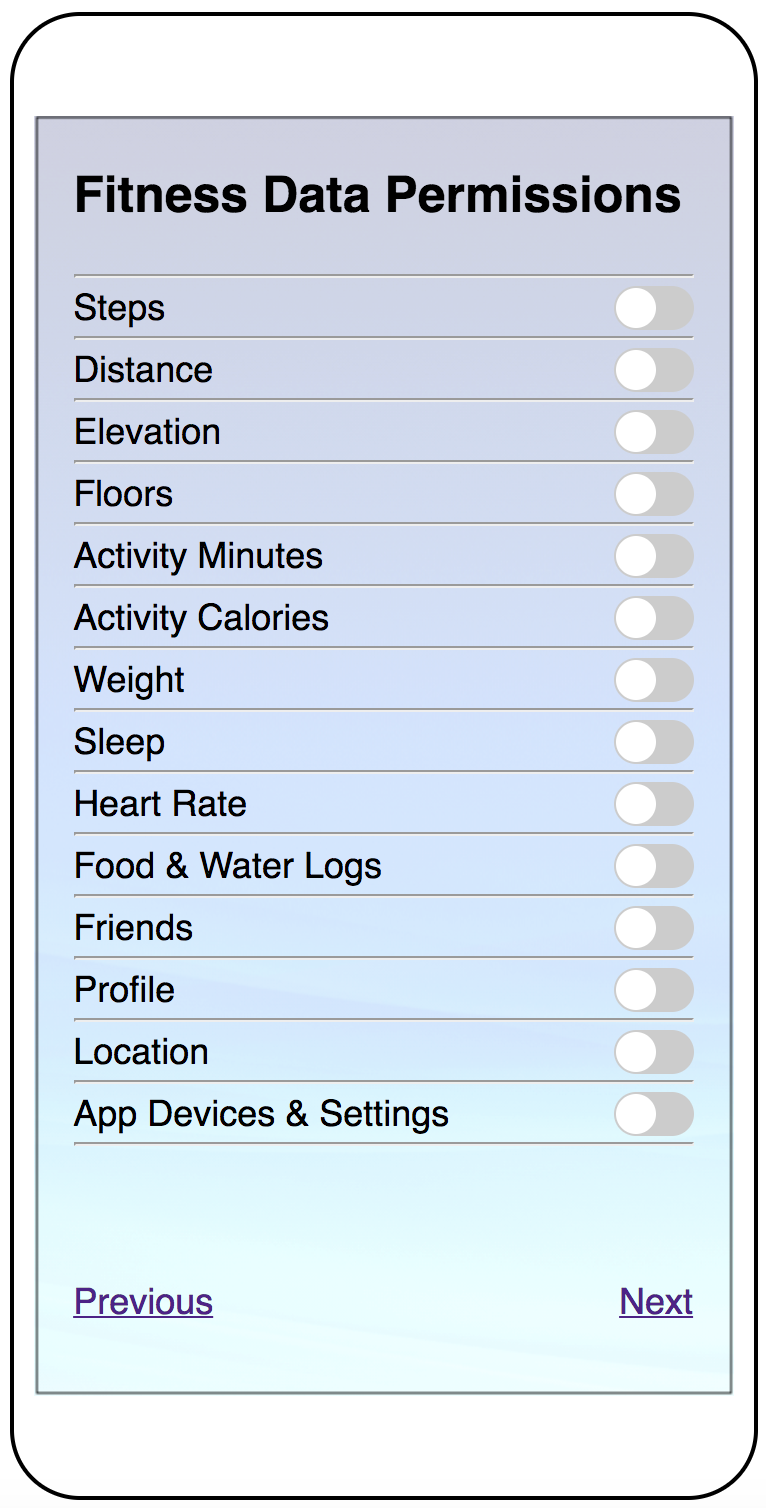
\includegraphics[width=0.24\textheight]{figures/manual2.png}
		\label{fig:manualb}
		\caption{F set}
	\end{subfigure}
	\begin{subfigure}[b]{0.24\textheight}
		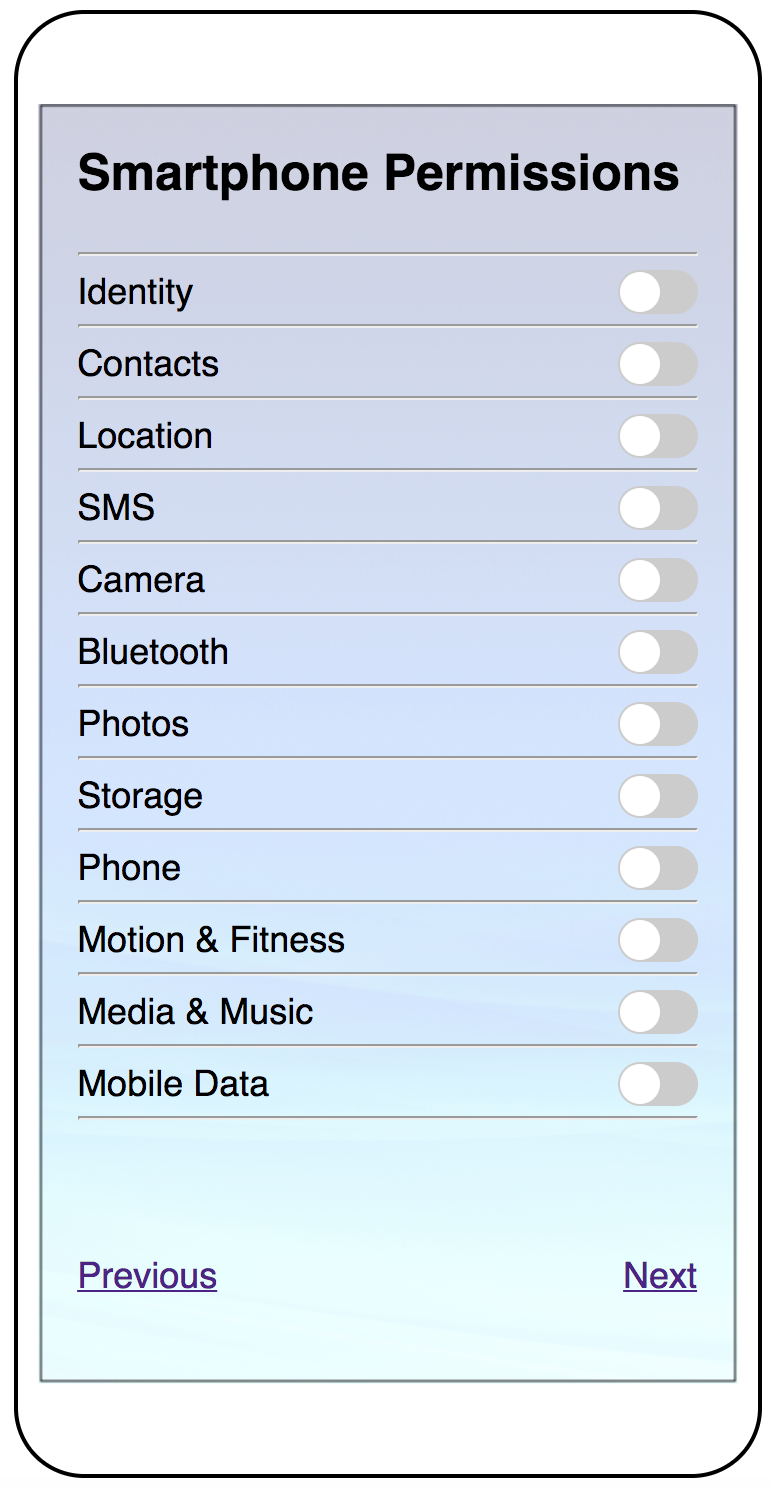
\includegraphics[width=0.24\textheight]{figures/manual3.png}
		\label{fig:manualc}
		\caption{S set}
	\end{subfigure}
	\begin{subfigure}[b]{0.24\textheight}
		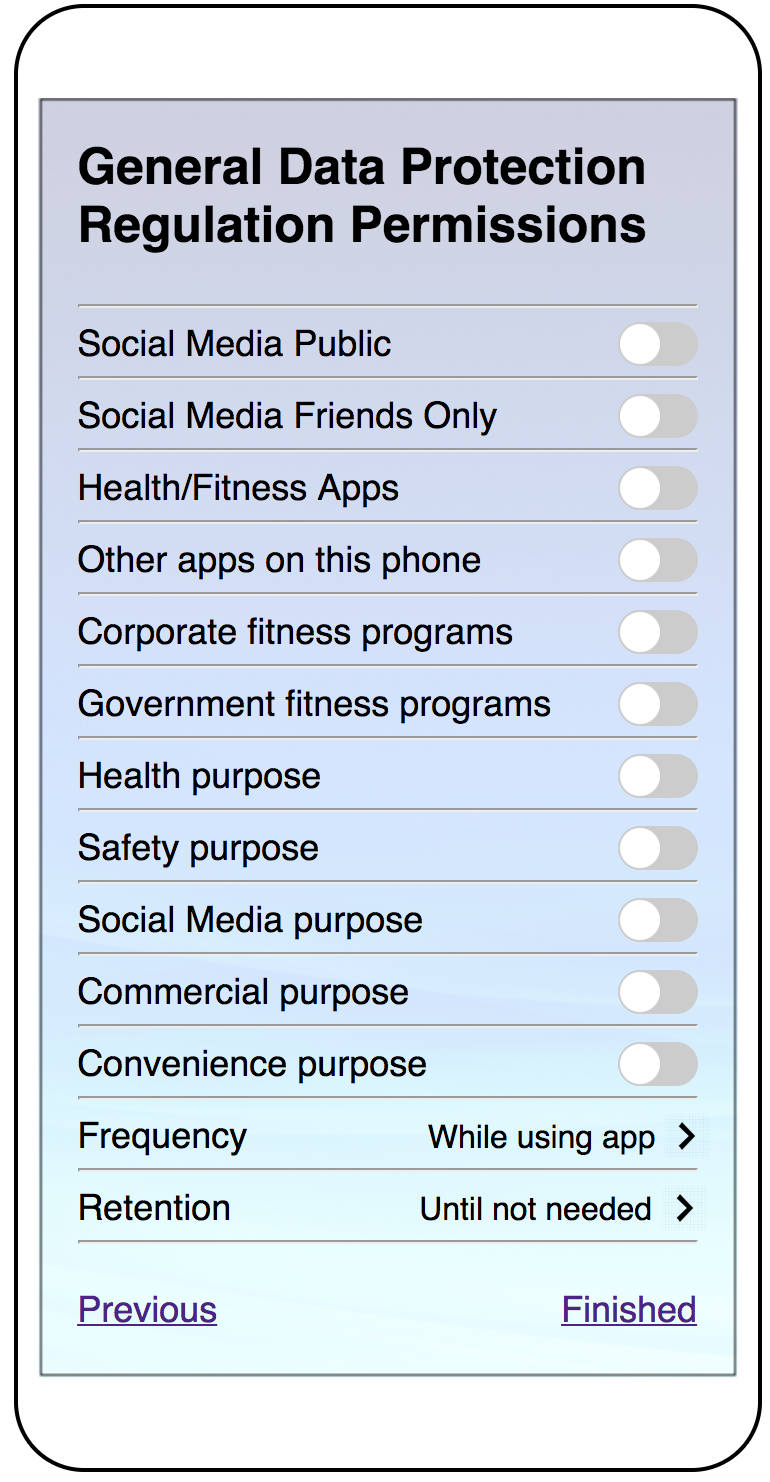
\includegraphics[width=0.24\textheight]{figures/manual4.png}
		\label{fig:manuald}
		\caption{G set}
	\end{subfigure}
	\caption{Manual settings}
	\label{fig:manual}
\end{figure}

%Ilaria
The next strategies exploit the results of the analysis in the previous section to provide \textit{interactive recommendations} that simplify the task of privacy permission setting, with different levels and type of user intervention.

%change to smart single --Prof.Ilaria
%I: No, I'd prefer Smart default, but since the online user interface is Smart single, it's ok like this too
\subsection{Single Smart Default Setting}

%In the case the user is tired, it is more likely that the user will just click accept on the default settings which is always all accept. Therefore, default manual has a lot of impact on the user's privacy preference.

One way to reduce the burden of privacy management is with single ``smart'' default setting. Rather than having the user set each permission manually, this solution already selects a default setting for each permission. Users can then review these settings and change only the ones that do not match their preferences.

The optimal ``smart'' default is a set of settings that is aligned with the preferences of the majority of users. Hence, we can calculate these setting by using the cluster centroid of the 1-cluster solution (i.e., the full dataset ``single cluster'' in Figure~\ref{fig:privacy_profiles}). Figure \ref{fig:default} shows the resulting default values for each dataset. If the user is unhappy with these settings, he/she can still make specific changes. Otherwise, he/she can keep them without making any changes. 

%% need change
%\begin{figure}[t]
%	\centering
%	\subfloat[A set]{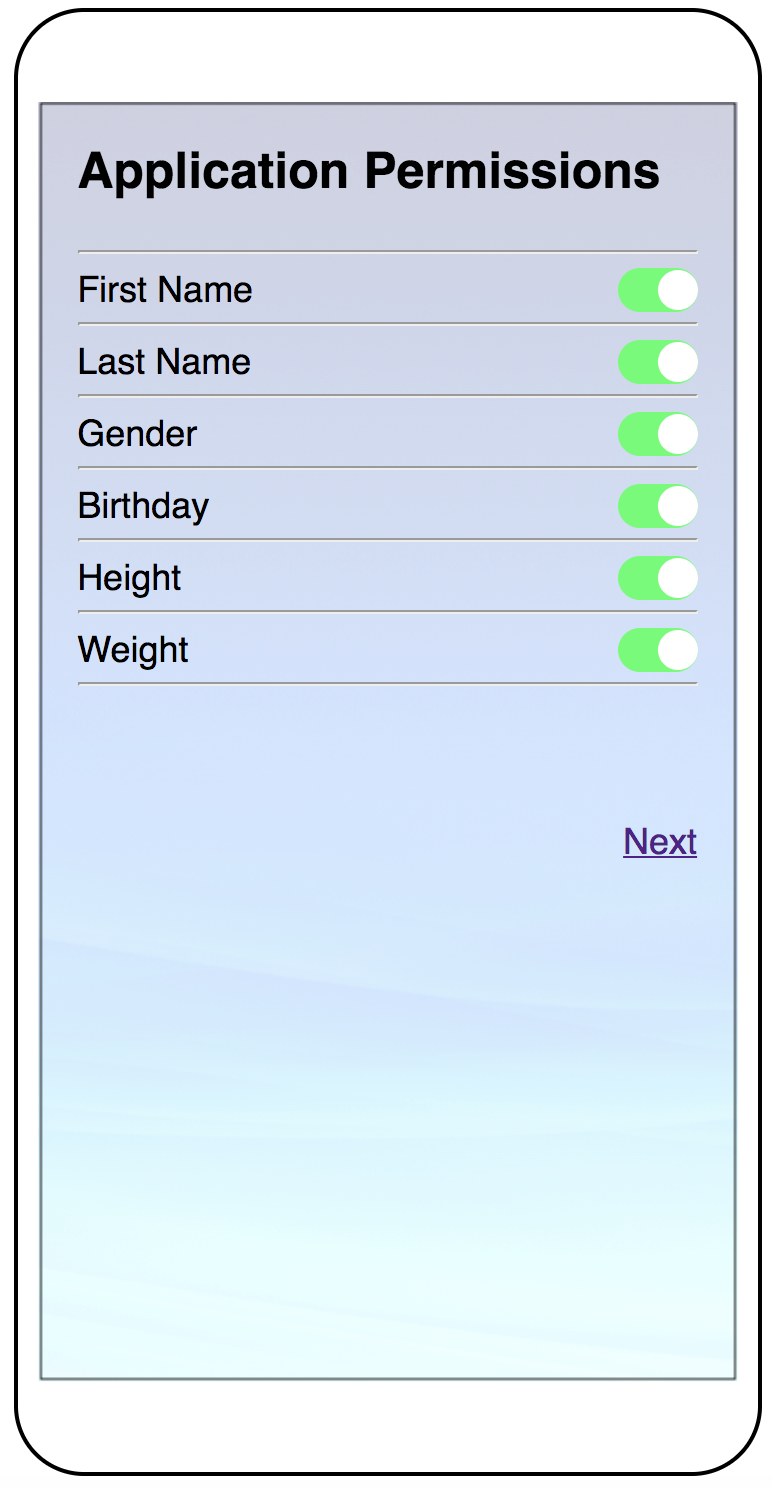
\includegraphics[width=0.36\linewidth]{figures/default1.png}\label{fig:defaulta}} \hspace{0.25cm}
%	\subfloat[F set]
%	{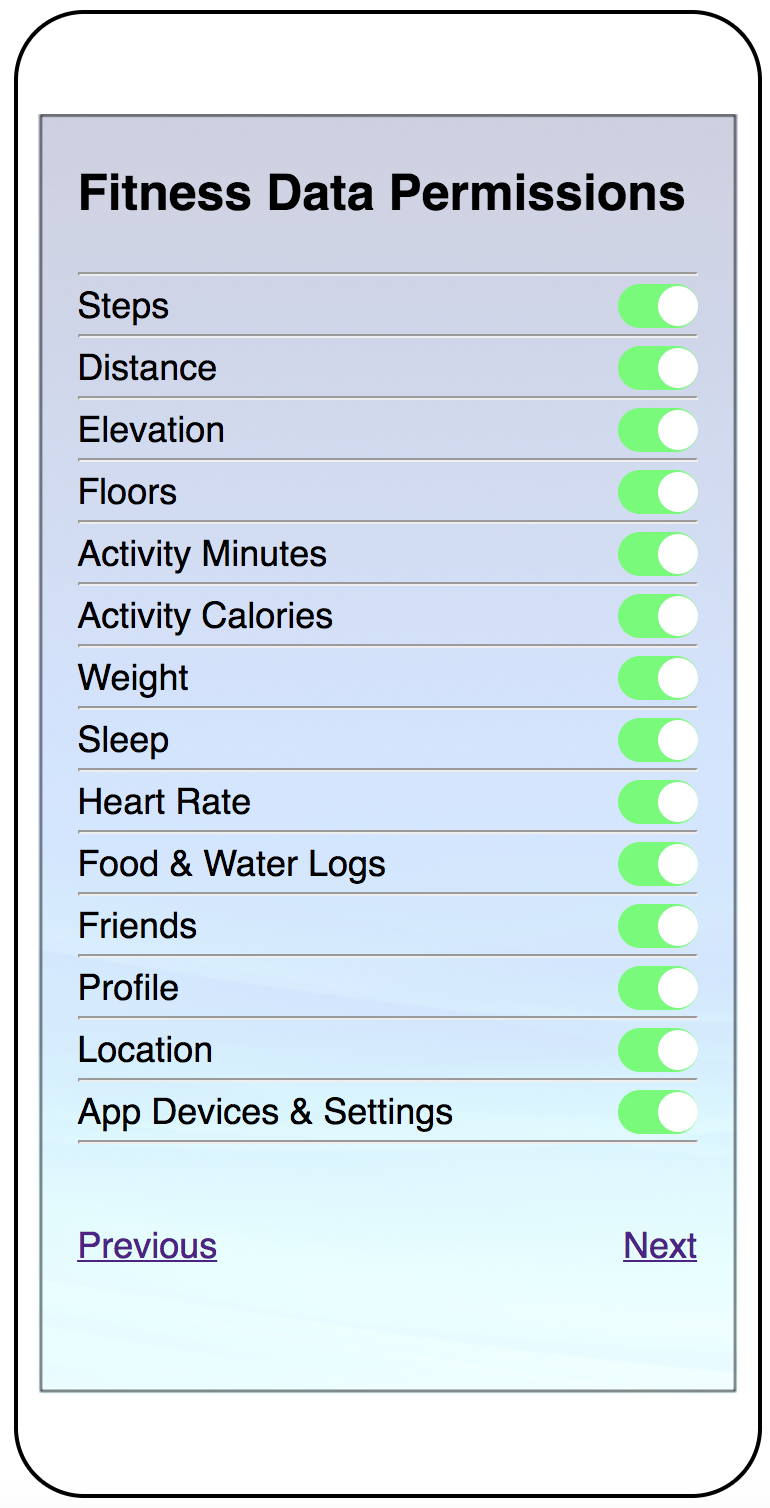
\includegraphics[width=0.36\linewidth]{figures/default2.png}\label{fig:defaultb}}
%	
%	\subfloat[S set]
%	{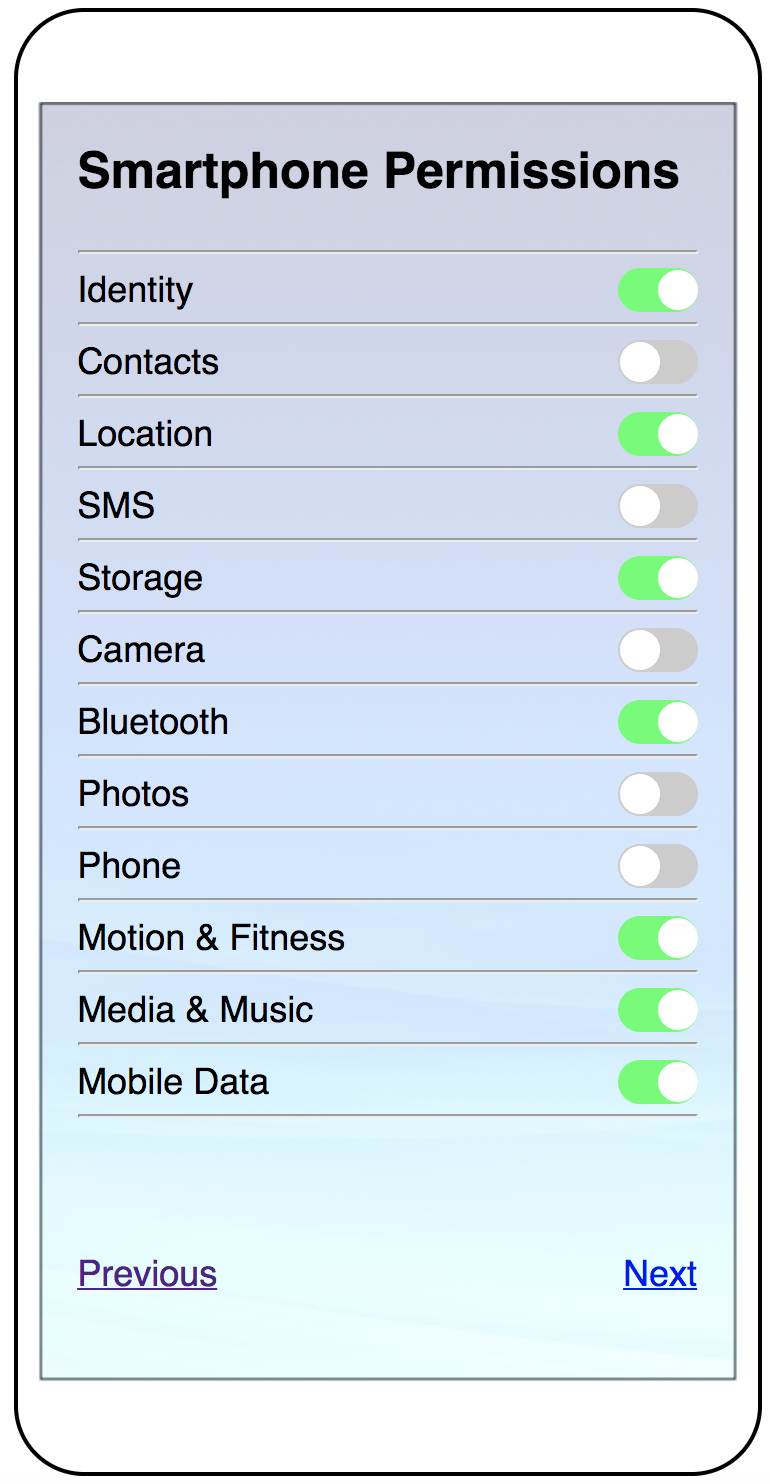
\includegraphics[width=0.36\linewidth]{figures/default3.png}\label{fig:defaultc}}
%	\hspace{0.25cm}
%	\subfloat[G set]{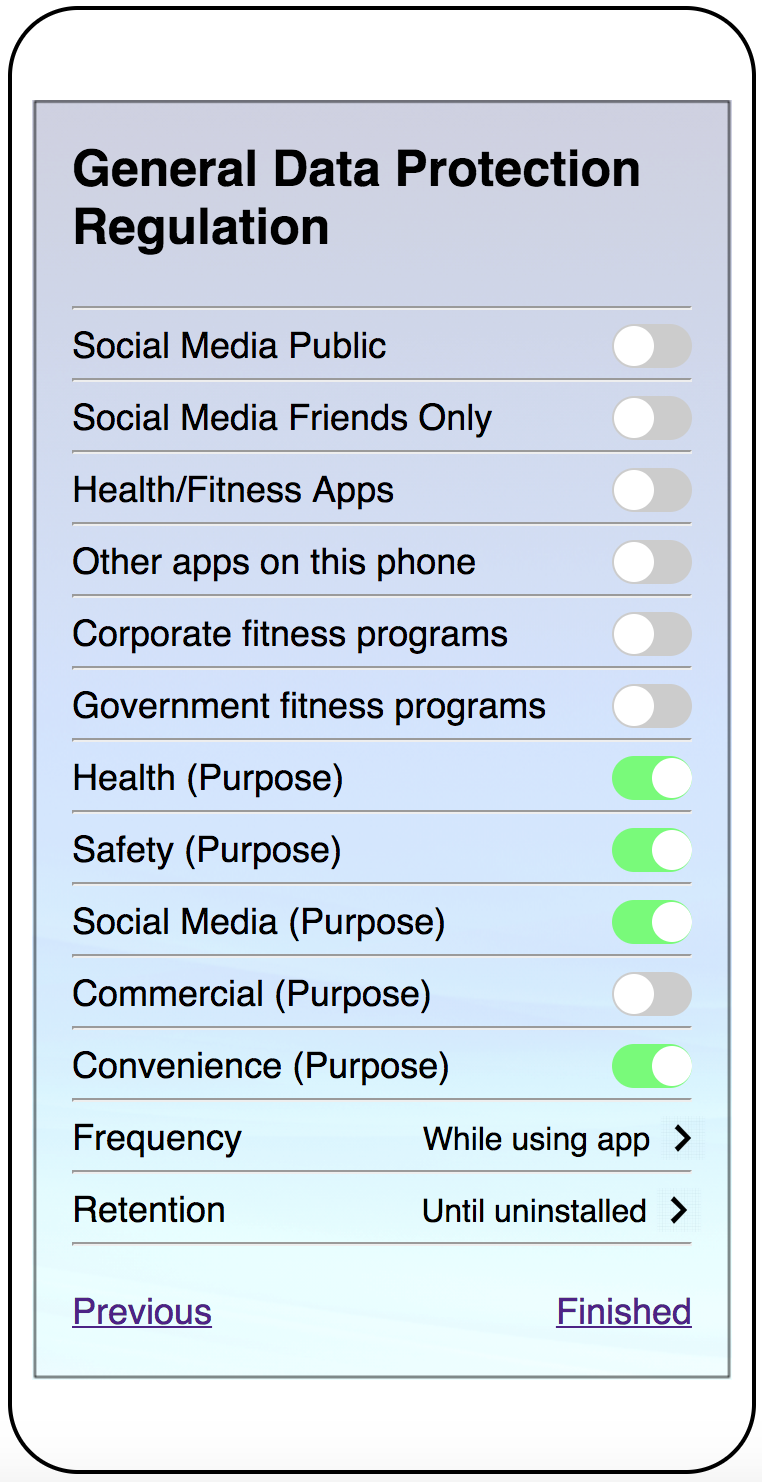
\includegraphics[width=0.36\linewidth]{figures/default4.png}\label{fig:defaultd}}
%	\caption{Smart Single settings.}
%	\label{fig:default}
%\end{figure}
\begin{figure}
	\centering
	\begin{subfigure}[b]{0.24\textheight}
		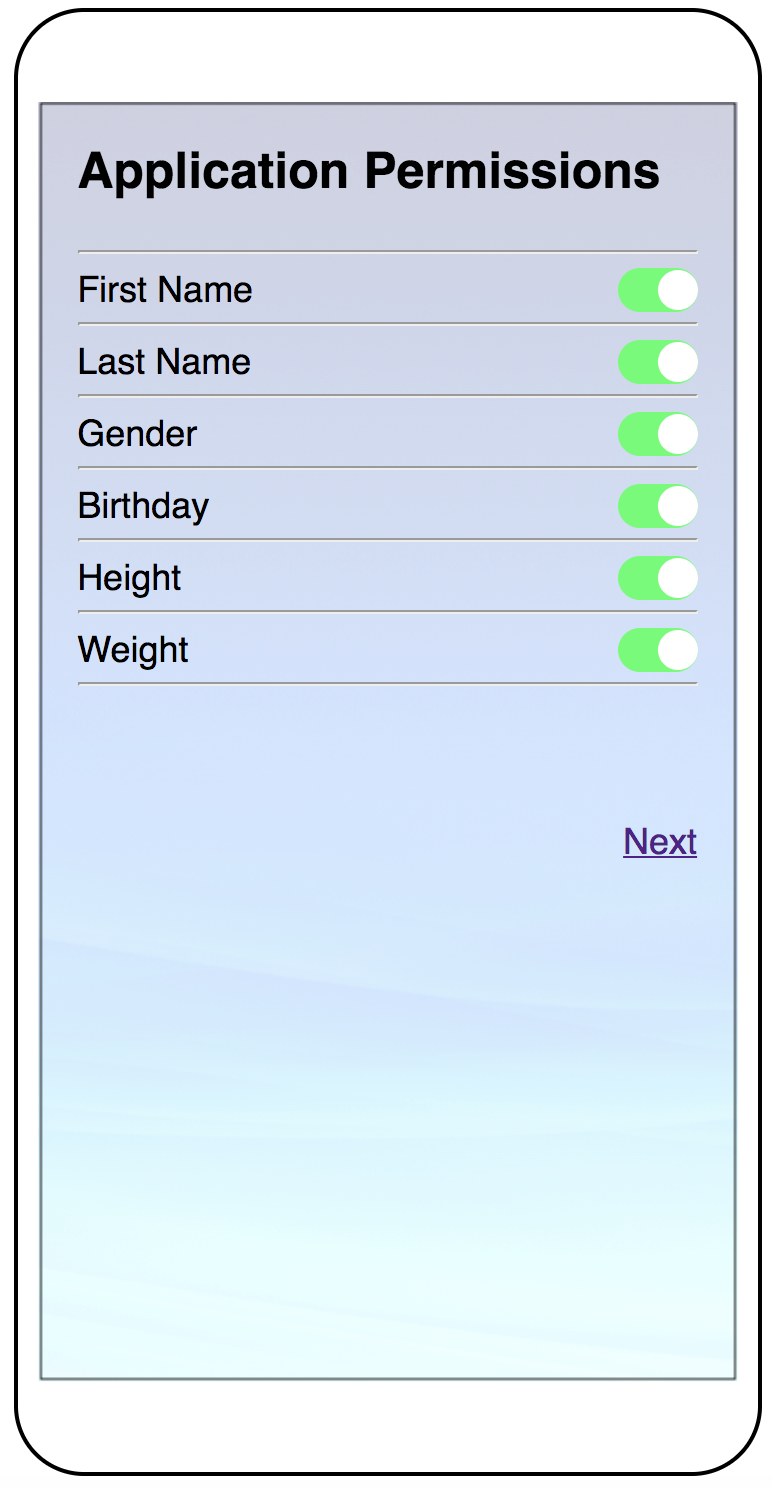
\includegraphics[width=0.24\textheight]{figures/default1.png}
		\label{fig:defaulta}
		\caption{A set}
	\end{subfigure}
	\begin{subfigure}[b]{0.24\textheight}
		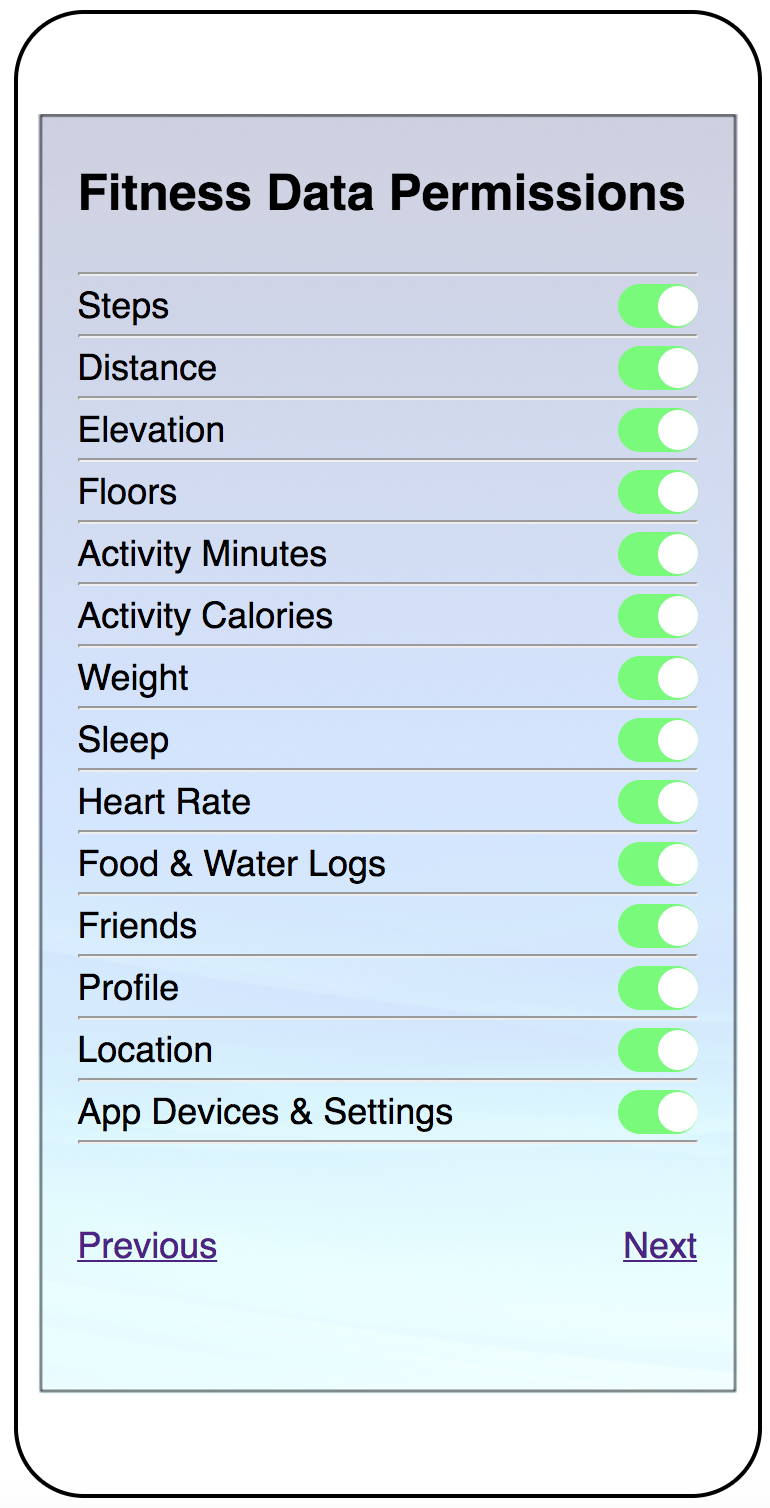
\includegraphics[width=0.24\textheight]{figures/default2.png}
		\label{fig:defaultb}
		\caption{F set}
	\end{subfigure}
	\begin{subfigure}[b]{0.24\textheight}
		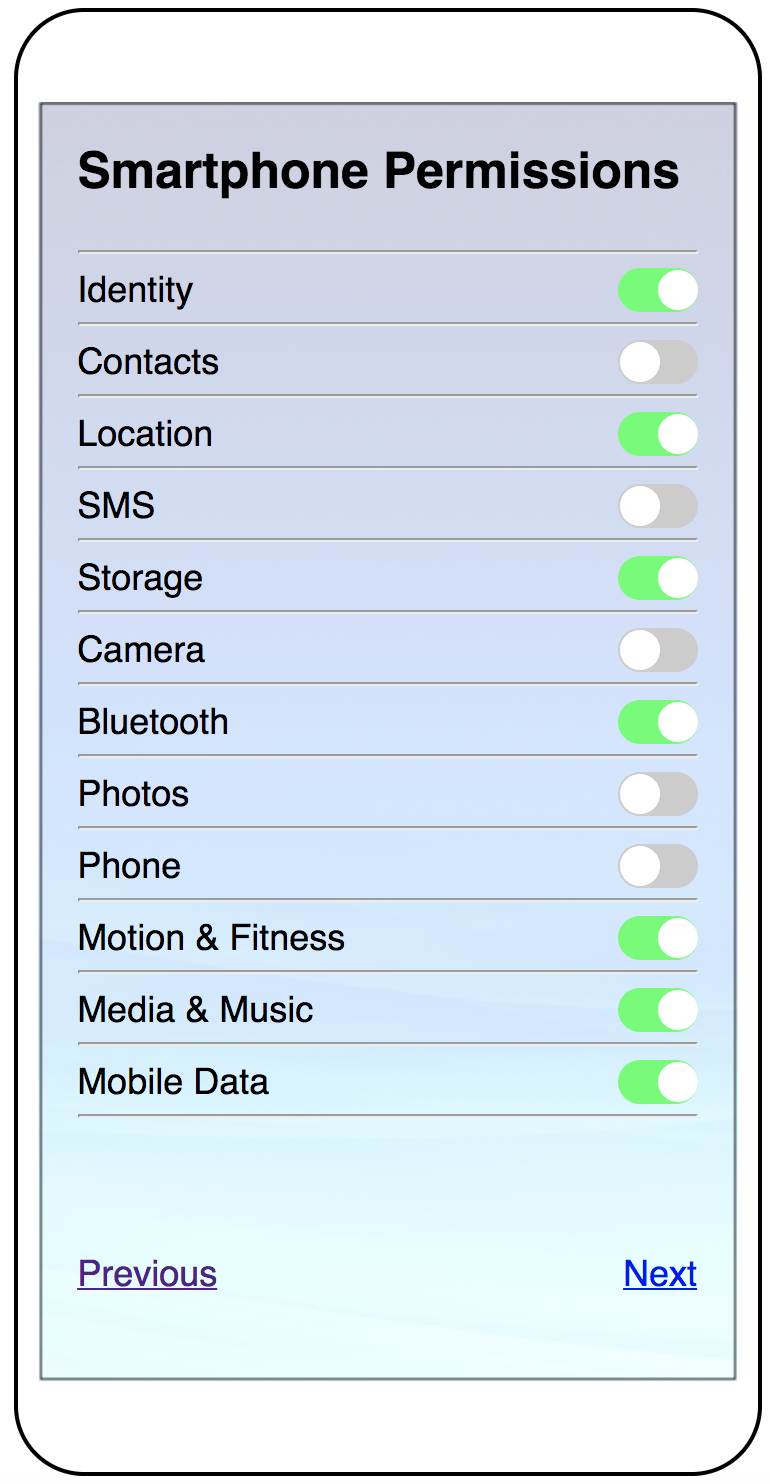
\includegraphics[width=0.24\textheight]{figures/default3.png}
		\label{fig:defaultc}
		\caption{S set}
	\end{subfigure}
	\begin{subfigure}[b]{0.24\textheight}
		\includegraphics[width=0.24\textheight]{figures/default4.png}
		\label{fig:defaultd}
		\caption{G set}
	\end{subfigure}
	\caption{Smart Single settings.}
	\label{fig:default}
\end{figure}


\subsection{Pick Subprofiles}

The single smart default setting works best when most users have preferences similar to the average. However, our dataset shows considerable variability in participants' privacy preferences---a finding that is broadly reflected in the privacy literature~\cite{knijnenburg2013dimensionality}. This bring us to our clustering solutions, which create \emph{separate} default settings (in the form of subprofiles) for distinct groups of users.

Our first approach in this regard is to have users manually select which privacy subprofiles they prefer. Figure~\ref{fig:pp} shows the subprofile selection interface for the S set. Users can choose either the ``Minimal'' or ``Unconcerned'' subprofile. Similar interfaces are provided for the F, A, and G sets.

The subprofiles provided by this approach have a higher overall accuracy than the single ``smart'' default described in Section~\ref{sec:manual}, meaning that the user could possibly spend less effort changing the settings. However, the user \emph{will} have to select a subprofile for each dataset. This highlights the importance of having a small number of subprofiles and making these subprofiles easy to understand. That said, even with only two subprofiles per dataset, this can be a challenging task. In the next two subsections, we address this problem by automatically selecting subprofiles based on users' answers to specific subprofile items (``direct prediction'') or questionnaire items (``indirect prediction'').

\begin{figure}
	\centering
	\begin{subfigure}[b]{0.22\textheight}
		\includegraphics[width=0.2\textheight]{figures/pickprofile.pdf}
		\label{fig:ppa}
		\caption{S set subprofiles}
	\end{subfigure}
~~
	\begin{subfigure}[b]{0.22\textheight}
		\includegraphics[width=0.2\textheight]{figures/pickprofile1.pdf}
		\label{fig:ppb}
		\caption{The ``Minimal'' subprofile}
	\end{subfigure}
~~
	\begin{subfigure}[b]{0.22\textheight}
		\includegraphics[width=0.2\textheight]{figures/pickprofile2.pdf}
		\label{fig:ppc}
		\caption{The ``Unconcerned'' subprofile}
	\end{subfigure}
	\caption{Interaction for picking a subprofile for the S set.}
	\label{fig:pp}
\end{figure}


\subsection{Direct Prediction}

For the direct prediction approach, we devise an interactive 4-question input sequence as shown in Figure \ref{fig:direct}. Each screen asks the user to answer a specific permission question, which guides the subprofile classification processes as outlined in Section~\ref{sec:direct}. In effect, each question informs the system about the user's subprofile of one of the four datasets, which means that users no longer have to manually pick the correct subprofiles. Specifically, users will be asked if they agree to share their First name (for the A set recommendation), Activity (for the F set), Photos (for the S set), and whether they allow their data to be used for Social purposes (for the G set). This 4-question interaction will aid the users in setting all of the 45 permissions in the system. Depending on the answer to these questions, the user will subsequently see the settings screens with the defaults set to the predicted profile. Users can still change specific settings if their preferences deviate from the selected profile.

%% need change
%\begin{figure}[t]
%	\centering
%	\subfloat[A set.]{\includegraphics[width=0.36\linewidth]{figures/direct1.png}\label{fig:directa}} \hspace{0.25cm}
%	\subfloat[F set.]
%	{\includegraphics[width=0.36\linewidth]{figures/direct2.png}\label{fig:directb}}
%	
%	\subfloat[S set.]
%	{\includegraphics[width=0.36\linewidth]{figures/direct3.png}\label{fig:directc}}
%	\hspace{0.25cm}
%	\subfloat[G set.]{\includegraphics[width=0.36\linewidth]{figures/direct4.png}\label{fig:directd}}
%	\caption{Direct Prediction questions.}
%	\label{fig:direct}
%\end{figure}
\begin{figure}
	\centering
	\begin{subfigure}[b]{0.24\textheight}
		\includegraphics[width=0.24\textheight]{figures/direct1.png}
		\label{fig:directa}
		\caption{A set}
	\end{subfigure}
	\begin{subfigure}[b]{0.24\textheight}
		\includegraphics[width=0.24\textheight]{figures/direct2.png}
		\label{fig:directb}
		\caption{F set}
	\end{subfigure}
	\begin{subfigure}[b]{0.24\textheight}
		\includegraphics[width=0.24\textheight]{figures/direct3.png}
		\label{fig:directc}
		\caption{S set}
	\end{subfigure}
	\begin{subfigure}[b]{0.24\textheight}
		\includegraphics[width=0.24\textheight]{figures/direct4.png}
		\label{fig:directd}
		\caption{G set}
	\end{subfigure}
	\caption{Direct Prediction questions.}
	\label{fig:direct}
\end{figure}




\subsection{Indirect Prediction}
\label{sec:indirect}

%% need change
%\begin{figure}[t]
%	\centering
%	\subfloat[A set.]{\includegraphics[width=0.36\linewidth]{figures/indirect1.png}\label{fig:indirecta}} \hspace{0.3cm}
%	\subfloat[F set.]
%	{\includegraphics[width=0.36\linewidth]{figures/indirect2.png}\label{fig:indirectb}}
%	
%	\subfloat[S set.]
%	{\includegraphics[width=0.36\linewidth]{figures/indirect3.png}\label{fig:indirectc}}
%	\hspace{0.3cm}
%	\subfloat[G set.]{\includegraphics[width=0.36\linewidth]{figures/indirect4.png}\label{fig:indirectd}}
%	\caption{Indirect Prediction questions.}
%	\label{fig:indirect}
%\end{figure}
\begin{figure}
	\centering
	\begin{subfigure}[b]{0.24\textheight}
		\includegraphics[width=0.24\textheight]{figures/indirect1.png}
		\label{fig:indirecta}
		\caption{A set}
	\end{subfigure}
	\begin{subfigure}[b]{0.24\textheight}
		\includegraphics[width=0.24\textheight]{figures/indirect2.png}
		\label{fig:indirectb}
		\caption{F set}
	\end{subfigure}
	\begin{subfigure}[b]{0.24\textheight}
		\includegraphics[width=0.24\textheight]{figures/indirect3.png}
		\label{fig:indirectc}
		\caption{S set}
	\end{subfigure}
	\begin{subfigure}[b]{0.24\textheight}
		\includegraphics[width=0.24\textheight]{figures/indirect4.png}
		\label{fig:indirectd}
		\caption{G set}
	\end{subfigure}
	\caption{Indirect Prediction questions.}
	\label{fig:indirect}
\end{figure}

For the indirect prediction approach, we take a similar approach, but the interactive 4-question input sequence is based on the analysis of questionnaire items rather than permission settings. 

As shown in Figure \ref{fig:indirect}, we selected 4 questions that yield the highest accuracy for each permission set: a negotiability question for Phone permissions for the S set, a negotiability question for the permission to share Sleep data for the F set, A question about sociability for the A set, and a trust question for the G set. %Bart: Isn't the negotiability question for the G set better? 
%ODNAN: Yes, but for the sake of diversity we chose the attitude, they only have decimal difference, we proposed this to you before
Negotiability and attitude have almost the same accuracy for G set, so we chose attitude for diversity.

The benefit of the indirect prediction approach is that the user does not have to answer any permission questions, not even the four needed to give a subprofile recommendation. Instead, the user has to answer four questionnaire items. 

%Combined accuracy now: 73.85 \%. S=neg, 74.44 A=hom,  F=neg, G=att.


\section{Validation}
We conducted a validation of these different approaches by running the recommendation strategies on the 30 users in our holdout dataset. The resulting recommended privacy subprofiles are then compared with their actual privacy preference. Figure~\ref{fig:aveaccuracy} shows the average accuracies of each of the presented approaches.

\begin{figure}[ht]
	\includegraphics[width=0.5\textheight]{figures/aveaccuracy4.png}
	\caption{Average accuracies of the recommender strategies on the holdout 30 users.}
	\label{fig:aveaccuracy}      
\end{figure}

%The evaluation has been performed for six categories, as shown in the figure. %\textit{Pick profile} can be used when the users pick the profiles themselves from the privacy profiles recommended to them. 
The \textit{Pick Profile} approach reaches an 84.74\% accuracy. This approach has the highest accuracy, because only the error from the difference between the privacy profile and the users' settings is counted, omitting the errors introduced by the user classification. This assumes that users can classify themselves with perfect accuracy---this is likely an incorrect assumption.

Among recommendation approaches, the \textit{direct prediction} approach is the most accurate, averaging 83.41\%. It almost yields no additional classification error compared to the \textit{Pick subprofile} approach. 
%%NEW UPDATE
%here is the explanation for the indirect
The \textit{indirect prediction} approach has a significantly lower accuracy of 73.9\%.
%All the indirect questions were combined from the highest accuracy for each set, negotiability for both S Set (74.44\%) and F Set (76.44\%), social behavior for A set (70.55\%), and attitude (72.3\%) for G set. Negotiability and attitude have almost the same accuracy for G set, so we chose attitude for diversity.


Finally, the \textit{single smart default} approach uses only a single ``profile'', circumventing the need for classification. The default profile settings are shown in the `full data' column of Figure \ref{fig:privacy_profiles}. The accuracy of this setting is lower than the accuracy of the subprofile solutions, but it does not lose accuracy on classification. Hence, its accuracy is a respectable 68.7\%, which is not much lower than the \textit{indirect prediction} approach. 

The details about accuracies are provided in Table~\ref{tab:allaccuracy} in Appendix.



% %\begin{tabular}{P{2cm}P{14cm}}
% \begin{table*}
% \centering
% % table caption is above the table
% \caption{Table of Accuracies from the User Evaluation.}
% \label{tab:allaccuracy}       % Give a unique label
% % For LaTeX tables use
% \newcolumntype{P}[1]{>{\arraybackslash}p{#1}}
% \begin{tabular}{P{2.5cm}P{1.7cm}P{2cm}P{1.5cm}P{1.5cm}P{1.9cm}P{1.9cm}}
% \hline\noalign{\smallskip}
%  %& \multicolumn{2}{c}{Baseline}  %\parbox{2.5cm}{Pick Profile\\ (Upper Bound)}
%  & Pick Profile (UB)  &  Smart Default (LB) & Direct questions & Attitude & Homophily Effect & Negotiability \\
% \noalign{\smallskip}\cmidrule(r){2-7}\noalign{\smallskip}



% \textit{S Set}\\
% \\
% Identity & 66.67\% & 66.67 \% &66.67 \%  & 66.67 \% &  66.67 \% & 66.67 \%\\
% Contacts & 83.33\% &70.00 \% &70.00 \% & 66.67 \% & 73.33 \%& 80 \%\\
% Location &83.33\% \%&83.33 \% &83.33 \% &  83.33 \% & 83.33 \%& 83.33 \%\\
% SMS  &90\% \%&50.00 \% & 70.00 \% & 60.00 \% & 53.33 \%& 73.33 \%\\
% Storage &83.33\% \%&56.67 \%&70.00 \%  & 53.33 \% & 46.67 \%& 60 \%\\
% Camera  &80\% \%&60.00 \% &86.67 \%  & 70.00 \% & 70.00 \% & 63.33 \%\\
% Bluetooth &83.33\% \% & 83.33 \% &83.33 \%  & 83.33 \% & 83.33 \% & 83.33 \%\\
% Photos &80\% \%&66.67 \%  &100 \%  & 76.66 \%  & 76.66 \%& 70 \%\\
% Phone & 96.67\% &56.67\% &76.67 \% & 66.67 \% & 60.00 \%& 80 \%\\
% Motion & 96.67\% & 96.67\% &96.67 \% & 96.67\% & 96.67\%& 96.67\%\\
% Media &70\%& 76.67\% &56.67 \% & 33.33\% & 33.33\%& 60.00 \%\\
% Mobile Data &76.67\% &76.67\% &76.67 \% & 76.67 \% & 76.67 \%& 76.67\%\\

% \cmidrule(r){2-7}
% Average & 82.5\%& 70.28 \% & 78.06 \% & 64.17\% & 68.33\% & 74.44\%\\
% \cmidrule(r){1-7}
% \textit{A set}\\
% \\

% First Name &100\% & 63.33 \% &100 \%& 63.33 \%& 73.33 \% & 56.67 \%\\
% Last Name &96.67 \%&60.00 \% &96.67 \%& 60.00 \%& 70 \% & 60 \%\\
% Gender &76.67 \%&76.67 \% & 76.67 \% & 76.67 \%& 76.67 \% & 76.67 \%\\
% Birthday &90.00 \%&60.00 \% &90.00 \%  & 60.00 \% & 63.33 \%& 53.33 \%\\
% Height &70.00 \%&70.00 \% & 70.00 \%& 70.00 \% & 70.00 \%& 70 \%\\
% Weight &70.00 \%&70.00 \% & 70.00 \%& 70.00 \%& 70.00 \%& 70 \%\\

% \cmidrule(r){2-7}
% Average & 83.89 \% & 66.67 \% & 83.89 \% & 66.67\% & 70.55\% & 64.44 \%\\ 
% \cmidrule(r){1-7}
% \textit{F set}\\
% \\
% steps &96.67 \%&73.33 \% &96.67 \%  & 76.67 \%& 70.00\% & 76.67\%\\
% distance &96.67 \%&73.33 \% &96.67 \% & 76.67 \% & 70.00\%& 76.67\%\\
% elevation &100 \%&70.00 \% &100 \% & 73.33 \% & 73.33\%& 80.00\%\\
% floors &96.67 \%& 73.33 \%&96.67 \% & 76.67 \% & 70.00\% & 76.67\%\\
% activity minutes &100 \%&70.00 \% &100 \% & 73.33 \% & 73.33\%& 80.00\%\\
% calories activity &96.67 \%&73.33 \% &96.67 \% & 76.67 \% & 70.00 & 76.67\%\\
% weight &90.00 \%&60.00 \% &90.00 \% & 63.33 \% & 70.00\%& 76.67\%\\
% sleep &93.33 \% &63.33 \% &93.33 \% & 66.67 \% & 66.67\% & 80\%\\
% heartrate &100 \% &70.00 \% &100 \% & 73.33 \% & 73.33\% & 80\%\\
% Food Logs &90 \% &60.00 \% &90.00 \% & 63.33 \% & 70.00\%& 76.67\%\\
% Friends &83.33 \% &53.33 \% &83.33 \% & 63.33 \% & 63.33\% & 70.00\%\\
% Profile &96.67 \% &66.67 \% &96.67 \% & 70.00\% &76.67\% & 76.67\%\\
% Location  &86.67 \% &56.67 \% &86.67 \% & 60.00 \% & 66.67\% & 66.67\%\\
% Device \& settings &93.33 \%  & 63.33 \% &93.33 \% & 66.67 \% & 73.33\% & 73.33\%\\

% \cmidrule(r){2-7}
% Average & 94.29 \%& 66.19 \% & 94.29 \% & 69.53\% &  70.48\% & 76.19\\
% \cmidrule(r){1-7}

% \textit{G set}\\
% \\
% SN Public &90.00 \% &90.00 \% &90.00 \%  & 90.00 \% &90.00 \%&90.00 \%\\
% SN Friends Only &73.33 \% &53.33 \% &73.33 \% & 63.33\% &60.00 \%&56.67 \%\\
% Health &66.67 \% &60.00 \% &60.00 \%  & 43.33\% &40.00 \%&70.00 \%\\
% Other Apps &76.67 \% &76.67 \% &76.67 \% & 76.67\% & 76.67 \%&76.67 \%\\
% Corporate &80.00 \% &80.00 \% &80.00 \% & 80.00\% & 80.00 \%&80.00 \%\\
% Government &86.67 \% & 86.67 \% &86.67 \% & 86.67\% & 86.67\%&86.67 \%\\
% Health &86.67 \% &86.67 \% &86.67 \% & 86.67 \% & 86.67\%&86.67 \%\\
% Safety &90.00 \% &90.00 \% &90.00 \%  & 90.00 \% & 90.00 \%&90.00 \%\\
% Social &93.33 \% &60.00 \% &100 \% & 70.00\% & 60.00 \%&63.33 \%\\
% Commercial & 73.33 \% & 73.33 \% &73.33 \% & 73.33 \% & 73.33 \%&73.33 \%\\
% Convenience & 80 \%& 73.33 \% &73.33 \% & 76.67\% & 66.67\%&70.00 \%\\
% Frequency & 53.33 \%& 53.33 \% &53.33 \% & 53.00 \% & 53.33 \%&53.33 \%\\
% Retention &50.00 \% &40.00\% &50.00 \% & 46.00 \% & 43.33 \%& 46.67 \%\\

% \cmidrule(r){2-7}
% Average & 76.92& 71.02 \% & 76.41 \% & 72.30 \% & 69.74 \%& 72.56\%\\
% \cmidrule(r){1-7}
% Over-all Average & 84.74\% & 68.74\% & 83.41\% & 70.07\% & 69.7\% & 73.11 \%  \\
% \end{tabular}
% \end{table*}

% \begin{table*}
% \centering
% % table caption is above the table
% \caption{Table of Accuracies from the User Evaluation.}
% \label{tab:trackers}       % Give a unique label
% % For LaTeX tables use
% \begin{tabular}{llllllll}
% \hline\noalign{\smallskip}
%  & \multicolumn{2}{c}{Baseline} & Initial & Attitude & Attitude & Attitude-to-trigger \\
%   &Upper Bound & Smart Default &4-q solution & 3-q solution & 4-q solution&1q &2q\\
% \noalign{\smallskip}\cmidrule(r){2-4}\noalign{\smallskip}



% \textit{phone Permissions}\\
% \\
% Identity & 66.67 & 66.67 \% &66.67 \% & 66.67 \% & 66.67 \%\\
% Contacts & 83.33 &70.00 \% &70.00 \% & 56.67 \% & 66.67 \%\\
% Location &83.33 \%&83.33 \% &83.33 \% & 83.33 \% & 83.33 \%\\
% SMS  &90 \%&50.00 \% & 70.00 \%& 50.00 \% & 66.67 \%\\
% Storage &83.33 \%&56.67 \%&70.00 \% & 43.33 \% & 66.67 \%\\
% Camera  &80 \%&60.00 \% &86.67 \% & 60.00 \% & 63.33 \%\\
% Bluetooth &83.33 \% & 83.33 \% &83.33 \% & 83.33 \% & 83.33 \% \\
% Photos &80 \%&66.67 \%  &100 \% & 60.00 \% & 56.66 \%\\
% Phone & 96.67\% &56.67\% &76.67 \% & 50.00 \%& 66.67 \%\\
% Motion & 96.67\% & 96.67\% &96.67 \% & 96.67\% & 96.67\%\\
% Media &70\%& 76.67\% &56.67 \% & 43.33 \% & 60.00\%\\
% Mobile Data &76.67\% &76.67\% &76.67 \% & 76.67 \% & 76.67 \%\\

% \cmidrule(r){2-4}
% Average & 82.5\%& 70.28 \% & 78.06 \% & 64.17\% & 71.11\% & 66.11\% & no sol. the same (66.11)\\
% \cmidrule(r){1-4}
% \textit{In-app Requests}\\
% \\

% First Name &100 & 63.33 \% &100 \%& 63.33 \%& \\
% Last Name &96.67 \%&60.00 \% &96.67 \%& 60.00 \%& \\
% Gender &76.67 \%&76.67 \% & 76.67 \% & 76.67 \%& \\
% Birthday &90.00 \%&60.00 \% &90.00 \%  & 60.00 \%&\\
% Height &70.00 \%&70.00 \% & 70.00 \%& 70.00 \%& \\
% Weight &70.00 \%&70.00 \% & 70.00 \%& 70.00 \%& \\

% \cmidrule(r){2-4}
% Average & 83.89 \% & 66.67 \% & 83.89 \% & 66.67\% & 66.67\% & (66.67 exp4) (66.67 trust4) (63.33 )(66.11 pc4) & (66.11 pv4+exp4) (66.11 trust4+pc4)\\
% \cmidrule(r){1-4}
% \textit{Fitness Data}\\
% \\
% steps &96.67 \%&73.33 \% &96.67 \%  & 76.67 \% \\
% distance &96.67 \%&73.33 \% &96.67 \% & 76.67 \% \\
% elevation &100 \%&70.00 \% &100 \% & 73.33 \%\\
% floors &96.67 \%& 73.33 \%&96.67 \% & 76.67 \% \\
% activity minutes &100 \%&70.00 \% &100 \% & 73.33 \%\\
% calories activity &96.67 \%&73.33 \% &96.67 \% & 76.67 \% \\
% weight &90.00 \%&60.00 \% &90.00 \% & 63.33 \% \\
% sleep &93.33 \% &63.33 \% &93.33 \% & 66.67 \% \\
% heartrate &100 \% &70.00 \% &100 \% & 73.33 \%\\
% Calorie intake &90 \% &60.00 \% &90.00 \% & 63.33 \%\\
% Friends &83.33 \% &53.33 \% &83.33 \% & 56.67\% \\
% Profile &96.67 \% &66.67 \% &96.67 \% & 70.00\% \\
% Location and GPS  &86.67 \% &56.67 \% &86.67 \% & 60.00 \%\\
% Device and settings &93.33 \%  & 63.33 \% &93.33 \% & 66.67 \%\\

% \cmidrule(r){2-4}
% Average & 94.29 \%& 66.19 \% & 94.29 \% & 69.53\% & same (69.53) (62.85 trust3) (70 trust4) & (69.52 trust4+sc1) (63.33 trust4+intrusion2) \\
% \cmidrule(r){1-4}

% \textit{G Dataset}\\
% \\
% \textit{Entities}\\
% Social Nets.\\ 
% -Public &90.00 \% &90.00 \% &90.00 \%  & 90.00 \% \\
% -Friends Only &73.33 \% &53.33 \% &73.33 \% & 63.33\% \\
% Health &66.67 \% &60.00 \% &60.00 \%  & 43.33\% \\
% Other Apps &76.67 \% &76.67 \% &76.67 \% & 76.67\%\\
% Fitness Programs\\
% -Corporate &80.00 \% &80.00 \% &80.00 \% & 80.00\%\\
% -Government &86.67 \% & 86.67 \% &86.67 \% & 86.67\%\\
% \textit{Purposes}\\
% -Health &86.67 \% &86.67 \% &86.67 \% & 86.67 \%\\
% -Safety &90.00 \% &90.00 \% &90.00 \%  & 90.00 \%\\
% -Social &93.33 \% &60.00 \% &100 \% & 70.00\%\\
% -Commercial & 73.33 \% & 73.33 \% &73.33 \% & 76.67 \%\\
% -Convenience & 80 \%& 73.33 \% &73.33 \% & 73.33\%\\
% Frequency & 53.33 \%& 53.33 \% &53.33 \% & 53.00 \%\\
% Retention &50.00 \% &40.00\% &50.00 \% & 46.00 \%\\

% \cmidrule(r){2-4}
% Average & 76.92& 71.02 \% & 76.41 \% & 72.30 \% & same (72.30\% trust1)  (72.82 trust4)& (70.51 pc4+sc1)\\
% \cmidrule(r){1-4}
% Over-all Average & 84.74\% & 68.74\% & 83.41\% & 68.52\% & 70.37\% final (attitude 70.67) , 71.56\% (attitude+influence)   \\
% \end{tabular}
% \end{table*}
%old solution
% A 67.22 96.67\% 3 cluster
% S 69.17 76.67\%
% F 66.19 94.29\%
% FIP 71.02 76.41\%
% Over-all=84.74\%

\section{Summary}
In this chapter, we have presented the following:

\begin{itemize}
	\item The dataset we used and Data modeling to fitness IoT permissions.
	\item Using a data-driven approach to developing user permission profiles
	\item A series of recommendation strategies that we developed for privacy management including direct prediction and more interestingly, indirect prediction using some user traits (users' privacy attitudes, the negotiability of their preferences, and social influence). 
\end{itemize}

One limitation of this work is that we have not tested the suitability of the recommendation strategies from the user's perspective. Specifically, we have conjectured that profile-based approaches reduce the hassle of making privacy settings but that the manual selection of a privacy profile might be difficult for a user. These conjectures should be evaluated in a user study, which we are currently working on.

In the next chapter, we discuss the evaluation study plan for our household IoT privacy-setting interface prototype.
